% This is  L2KURZ.TEX - LaTeX2e Kurzbeschreibung v2.x, Erlangen 1998, 1999
% This was L2KURZ.TEX - LaTeX2e Kurzbeschreibung, Mainz 1994,1995
% This was LKURZ.TEX - LaTeX Kurzbeschreibung, Uni Graz & TU Wien, 1987.
% last changes: 1999-04-18 WaS
%
\newcommand{\lkver}{2.1}             % laufende Versionsnummer ...
\newcommand{\lkdate}{18. April 1999} % ... und Datum
%
% Um die LaTeX-Kurzbeschreibung zu formatieren, benoetigen Sie LaTeX2e
% (in der Version vom Juni 1998 oder neuer) und folgende Dateien:
%
%      l2kurz.tex (diese Datei),
%      l2k1.tex, l2k2.tex, l2k3.tex, l2ksym.tex, 
%      l2k4.tex, l2k5.tex, l2k6.tex, l2ka.tex, a.ps,
%      german.sty (Version 2.5d oder neuer), latexsym.sty,
%      textcomp.sty, alltt.sty, graphics.sty
%
% LaTeX2e muss ueber die "traditionellen" deutschen Trennmuster
% dehypht.tex (von N. Schwarz, Bochum, 1993/1994) verfuegen..
%
% Bitte senden Sie Aenderungswuensche und Hinweise auf Fehler an
% Walter Schmidt <walter.schmidt@arcormail.de>.
% ----------------------------------------------------------------------

\documentclass[11pt,a4paper]{article} % ergaenze `twoside', wenn gewunscht!
\NeedsTeXFormat{LaTeX2e}[1998/06/01]  % wegen \mathring und Textsymbolen

\typeout{   Copyright 1998, 1999 W.Schmidt, J.Knappen, H.Partl, I.Hyna   }
\typeout{   Copyright 1994, 1995 J.Knappen, H.Partl, E.Schlegl, I.Hyna   }
\typeout{   Copyright 1987 H.Partl, E.Schlegl, I.Hyna                    }

\usepackage{german,latexsym,alltt}
\usepackage[dvips,draft]{graphics} 
% Eine ps-Datei muss gelesen werden, aber die dvi-Datei soll mit jedem 
% dvi-Treiber, auch ohne PostScript-Unterstuetzung, zu verarbeiten sein!

% Sind die TC-Fonts vorhanden?
\newif\iftcfonts\tcfontstrue
\def\checkfont#1{%
  \batchmode
  \font\test=#1\relax
  \errorstopmode
  \ifx\test\nullfont
    \tcfontsfalse
  \fi}
\checkfont{tcrm1095}

% Wenn ja, dann lade textcomp.sty:
\iftcfonts\usepackage{textcomp}\fi

% Texthoehe 46 Zeilen + \topskip
% (Rand ueber der Kopfzeile) : (Rand unter dem Text) = 1:2
%
\setlength{\textheight}{46\baselineskip}
\addtolength{\textheight}{\topskip}
\newlength{\uppermargin}
\setlength{\uppermargin}{\paperheight}
\addtolength{\uppermargin}{-\textheight}
\addtolength{\uppermargin}{-\headsep}
\addtolength{\uppermargin}{-\headheight}
\setlength{\uppermargin}{.333\uppermargin} % Raender oben/unten 1:2
\addtolength{\uppermargin}{-1in}
\setlength{\topmargin}{\uppermargin}
%
% Textbreite 5.2in
% Text hor. zentriert
%
\setlength{\textwidth}{5.2in}
\setlength{\oddsidemargin}{.5339in}
\setlength{\evensidemargin}{\oddsidemargin}
%

% Seitenzahlen oben, aber keine Kopfzeile
\pagestyle{myheadings}
\markboth{}{}

%
\renewcommand{\textfraction}{.1}      % Make float placement easier
\renewcommand{\floatpagefraction}{.7}


\newcommand{\bs}{\symbol{92}} % Ein Backslash in Schreibmaschinenschrift;
                              % nur mit OT1-Fonts zu verwenden!
\makeatletter
%
% \path aus dtk.sty ( heisst dort \Path )
\begingroup
\gdef\path@SepI{/""}
\gdef\path@SepII{\symbol{92}""}
\gdef\path@SepIII{:""}
\catcode`\/=13
\catcode`\:=13
\catcode`\^=0
^catcode`\\=13
^gdef^path{^begingroup
  ^catcode`^/=13 
  ^catcode`^\=13 
  ^catcode`^:=13 
  ^catcode`^~=12 
  ^catcode`^$=12 %$
  ^catcode`^_=12 
  ^catcode`^#=12 
  ^let/=^path@SepI
  ^let\=^path@SepII
  ^let:=^path@SepIII
  ^@path}
^gdef^@path#1{^texttt{#1}^endgroup}
^endgroup
%
% LaTeXe-Symbol fuer cmss/sbc mit groesserem Absstand L-a und halbfettem Epsilon
\DeclareRobustCommand{\sbLaTeXe}{{\fontseries{sbc}\selectfont\boldmath%
        L\kern-.25em% -.36
        {\sbox\z@ T%
         \vbox to\ht\z@{\hbox{\check@mathfonts
                              \fontsize\sf@size\z@
                              \math@fontsfalse\selectfont
                              A}%
                        \vss}%
        }%
        \kern-.15em%
        \TeX\kern.15em2$_{\textstyle\varepsilon}$}}
%        
\makeatother

\newcommand\exa{\nopagebreak \begin{flushleft}\smallskip \nopagebreak
                \begin{minipage}[t]{6cm}\sloppy}
\newcommand\exb{\end{minipage}\kern 1cm\begin{minipage}[t]{8cm}\sloppy }
\newcommand\exc{\end{minipage}\kern -3cm \smallskip\end{flushleft}}
 
\newcommand\oben[1]{\begin{center}\begin{minipage}{#1}\hrule\medskip}
\newcommand\unten  {\hrule \end{minipage}\end{center}}

\newenvironment{ttdescription}{%
  \renewcommand{\descriptionlabel}[1]{%
    \hspace{\labelsep}\texttt{##1}}%
  \begin{description}%
}{%
  \end{description}%
}

\newcommand{\manual}{\emph{\LaTeX-Handbuch}~\cite{manual}}
\newcommand{\local}{\emph{Local Guide}~\cite{local}}

\newenvironment{symbols}{%
   \begin{tabbing}
   \hspace{1cm}\=\hspace{3.5cm}\=  \hspace{1cm}\=\hspace{3.5cm}\=
   \hspace{1cm}\=\hspace{3.5cm}\=  \kill
   }{%
   \end{tabbing}}

\newcommand{\nfrac}[2]{\leavevmode\kern.1em%
  \raise.5ex\hbox{\scriptsize #1}%
  \kern-.1em/\kern-.15em%
  \lower.25ex\hbox{\scriptsize #2}}

\nonfrenchspacing      % german.sty sets frenchspacing automatically.
%  However, some examples are pointless with frenchspacing in action. 
%  Besides, the larger space after a sentence make the text more readable.


\begin{document}

\begin{titlepage} % <-------- neue Titelseite
\renewcommand{\thefootnote}{\fnsymbol{footnote}}
{\Huge%
\fontfamily{cmss}\fontseries{sbc}\selectfont
\raggedright
\sbLaTeXe-Kurzbeschreibung
\rule{\textwidth}{0.75pt}
\par
}
\begin{flushleft}
  \normalsize
  \fontfamily{cmss}\fontseries{sbc}\selectfont
  Version \lkver\\
  \lkdate\\[2ex]
  Walter Schmidt\footnote{%
    Erlangen, \texttt{<walter.schmidt@arcormail.de>}}\\
  J"org Knappen\footnote{%
    Electronic Technologies, Springer-Verlag, Heidelberg}\\
  Hubert Partl\footnote{%
    Zentraler Informatikdienst der Universit"at f"ur Bodenkultur, Wien}\\
  Irene Hyna\footnote{%
    Bundesministerium f"ur Wissenschaft und Verkehr, Wien}
\end{flushleft}

\vfill

{\parindent=0cm
\LaTeX{} ist ein Satzsystem, das f"ur viele Arten von
Schrift"-st"u"cken verwendet werden kann, von einfachen Briefen bis zu
kompletten B"uchern.  Besonders geeignet ist es f"ur 
wissenschaftliche oder technische Dokumente. \LaTeX{} ist f"ur 
praktisch alle verbreiteten Betriebssysteme verf"ugbar.
 
Die vorliegende Kurzbeschreibung bezieht sich auf die Version
\LaTeXe\ in der Fassung vom 1.\ Juni~1998 und sollte f"ur den 
Einstieg in \LaTeX{} ausreichen.  
Eine voll"-st"andige Beschreibung ent"-h"alt das \manual{}
in Verbindung mit der Online-Dokumentation.
}
\setcounter{footnote}{0}
\end{titlepage}

%\newpage

{\parindent=0cm\thispagestyle{empty}
\copyright{} Copyright 1998, 1999 W.~Schmidt, J.~Knappen, H.~Partl, I.~Hyna
\bigskip

Die Verteilung dieses Dokuments in elektronischer oder gedruckter
Form ist gestattet, solange sein Inhalt einschlie"slich Autoren- und 
Copyright-Angabe unver"andert bleibt und die Verteilung kostenlos
erfolgt, abgesehen von einer Ge\-b"uhr f"ur den Datentr"ager, den
Kopiervorgang usw.
\bigskip

Die in dieser Publikation erw"ahnten Software- und Hardware-Bezeichnungen sind
in den meisten F"allen auch eingetragene Warenzeichen und unterliegen als
solche den gesetzlichen Bestimmungen.
\bigskip

\vfill

Dieses Dokument wurde mit \LaTeX{} gesetzt.
Sein Quelltext ist zu finden unter
\path{<ftp://ftp.dante.de/tex-archive/info/lshort/german/>}.
\bigskip

Die Autoren danken Michael Hofmann, Rainer Sch"opf, Stefan 
Steffens, Luzia Dietsche, Bernd Raichle und Heiko Oberdiek 
f"ur Tips, Anmerkungen 
und  Korrekturen.
}

\newpage

\setcounter{page}{1}
\tableofcontents

\newpage
 
% master: l2kurz.tex
% L2K1.TEX - 1.Teil der LaTeX2e-Kurzbeschreibung v2.x, Erlangen 1998, 1999
% L2K1.TEX - 1.Teil der LaTeX2e-Kurzbeschreibung Mainz 1994, 1995
% LK1.TEX  - 1.Teil der LaTeX-Kurzbeschreibung Graz-Wien 1987
% last changes: 1999-04-18 WaS


\section{Allgemeines}
 
% Note: the large number of short subsubsections in this section
% helps to avoid pages full of text (without any white space),
% which would look bad and might cause a `page memory overflow' on
% some printers like the XEROX 2700.
 
\subsection{The Name of the Game}
 
\subsubsection{\TeX}

\TeX\ (sprich "`Tech"', kann auch "`TeX"' geschrieben werden) ist
ein Computer\-progamm von Donald E.~Knuth~\cite{texbook,schwarz}.
Es dient zum Setzen und Drucken von Texten und mathematischen
Formeln.
 
\subsubsection{\LaTeX}
 
\LaTeX\ (sprich "`Lah-tech"' oder "`Lej-tech"', kann auch
"`LaTeX"' geschrieben werden) ist ein auf \TeX\ auf\/bauendes Computerprogramm
und wurde von Leslie Lamport~\cite{manual,wonne} geschrieben.
Es vereinfacht den Umgang mit \TeX, indem es 
entsprechend der logischen Struktur des Dokuments auf vorgefertigte
Layout-Elemente zur"uckgreift.

\subsubsection{\LaTeXe}

\LaTeXe\ (sprich "`\LaTeX\ zwei e"') ist die aktuelle Variante von
\LaTeX\ seit dem 1.~Juni 1994.  (Die vorherige hie"s \LaTeX~2.09.)
Wenn hier von \LaTeX\ gesprochen wird, so ist normalerweise dieses
\LaTeXe{} gemeint.

Neue Versionen  % <---------- bessere Formulierung?
von \LaTeXe{} (z.\,B. mit Fehlerberichtigungen oder Er\-g"an\-zun\-gen)
erscheinen zweimal j"ahrlich im Juni und im 
Dezember; die vorliegende Beschreibung setzt mindestens diejenige
vom Juni 1998 voraus.  

\subsection{Grundkonzept}
 
\subsubsection{Autor, Designer und Setzer}
 
F"ur eine Publikation "ubergab der Autor dem Verleger
traditionell  ein maschinengeschriebenes Manuskript.  Der
Buch-Designer des Verlages entschied dann "uber das Layout des
Schrift"-st"ucks (L"ange einer Zeile, Schriftart, Ab\-st"ande vor
und nach Kapiteln usw.\@) und schrieb dem Setzer die
daf"ur notwendigen Anweisungen dazu.
%--- Somit ist das gesetzte Schrift"-st"uck
%--- das Ergebnis des Buch-Designers und nicht des Autors.
\LaTeX{} ist in diesem Sinne der Buch-Designer, 
das Programm \TeX{} ist sein Setzer.
 
Ein menschlicher Buch-Designer erkennt die Absichten des Autors
(z.\,B.\ Kapitel-"Uberschriften, Zitate, Beispiele, Formeln
\dots) meistens aufgrund seines Fachwissens aus dem Inhalt des
Manuskripts.  \LaTeX{} dagegen ist "`nur"' ein Programm und
ben"otigt daher zus"atzliche Informationen vom Autor, die die
logische Struktur des Textes beschreiben.
Diese Informationen werden in Form von sogenannten "`Befehlen"'
innerhalb des Textes angegeben.
Der Autor braucht sich also
(weitgehend) nur um die logische Struktur seines Werkes zu k"ummern,
nicht um die Details von Gestaltung und Satz.
 
Im Gegensatz dazu steht der visuell orientierte Entwurf eines
Schrift"-st"u"ckes mit Textverarbeitungs- oder DTP-Programmen wie z.\,B.\ 
\textsc{Word}.
In diesem Fall legt der Autor das Layout des Textes gleich bei der
interaktiven Eingabe fest. Dabei sieht er am Bildschirm das, was
auch auf der gedruckten Seite stehen wird. Solche Systeme, die das
visuelle Entwerfen unter"-st"utzen, werden auch WYSIWYG-Systeme
("`what you see is what you get"') genannt.
 
Bei \LaTeX{} sieht der Autor beim Schreiben des Eingabe"-files in
der Regel noch nicht sofort, wie der Text nach dem Formatieren 
aussehen wird. Er kann aber %durch Aufruf des entsprechenden Programms 
jederzeit einen "`Probe-Ausdruck"' seines Schrift"-st"ucks auf dem
Bildschirm machen und danach sein Eingabe"-file entsprechend 
korrigieren und die Arbeit fortsetzen.
 
 
\subsubsection{Layout-Design}
 
Typographisches Design ist ein Handwerk, das erlernt werden mu"s.
Unge"-"ubte Autoren machen oft gravierende Formatierungsfehler.
F"alsch"-licherweise glauben viele Laien, da"s Textdesign
vor allem eine Frage der "Asthetik ist -- wenn das
Schrift"-st"uck vom k"unstlerischen Standpunkt aus "`sch"on"'
aussieht, dann ist es schon gut "`designed"'.
Da Schrift"-st"u"cke jedoch gelesen und nicht in einem Museum
auf"-ge"-h"angt werden, sind die leichtere Lesbarkeit und bessere
Ver"-st"and"-lichkeit wichtiger als das sch"one Aussehen.
 
Beispiele:
Die Schrift"-gr"o"se und Numerierung von "Uberschriften soll so
ge"-w"ahlt werden, da"s die Struktur der Kapitel und Unterkapitel
klar erkennbar ist.
Die Zeilen"-l"ange soll so ge"-w"ahlt werden, da"s anstrengende
Augenbewegungen des Lesers vermieden werden, nicht so, da"s der
Text das Papier m"oglichst sch"on aus"-f"ullt.
 
Mit interaktiven visuellen Entwurfssystemen ist es leicht,  
% "asthetisch sch"one, aber schlecht strukturierte
%-----  falsch: nur die Darstellung ist schlecht, 
%-----  die Strukturierung ist vielleicht ok.
Schrift"-st"u"cke zu erzeugen, die zwar "`gut"' aussehen,
aber ihren Inhalt und dessen Aufbau nur mangelhaft wiedergeben.
\LaTeX{} verhindert solche
Formatierungsfehler, indem es den Autor dazu zwingt, die logische
Struktur des Textes anzugeben, und dann automatisch ein da"-f"ur
geeignetes Layout verwendet.

Daraus ergibt sich, da"s \LaTeX{} insbesondere f"ur  Dokumente geeignet 
ist, wo vorgegebene Gestaltungsprinzipien auf sich wiederholende
logische Textstrukturen angewandt werden sollen. 
F"ur das -- notwendigerweise -- visuell orientierte Gestalten
etwa eines Plakates ist \LaTeX{} hingegen 
aufgrund seiner Arbeitsweise weniger geeignet.

\subsubsection{Vor- und Nachteile}

Gegen"uber anderen Textverarbeitungs- oder DTP-Programmen 
zeichnet sich \LaTeX{}
vor allem durch die folgenden Vorteile aus:
\begin{itemize}
\item Der Anwender mu"s nur wenige, leicht verst"andliche Befehle
  angeben, die die logische Struktur des Schrift"-st"ucks
  betreffen, und braucht sich um die gestalterischen Details
  (fast) nicht zu k"ummern.
\item Das Setzen von mathematischen Formeln ist besonders gut
  unter"-st"utzt.
\item Auch anspruchsvolle Strukturen wie Fu"snoten, Literaturverzeichnisse,
  Tabellen u.\,v.\,a.\  k"on"-nen mit wenig Aufwand erzeugt werden.
% ---- schwammige Formulierung ;-)
\item Routineaufgaben wie das Aktualisieren von Querverweisen
 oder die Erstellung des Inhaltsverzeichnisses 
 werden automatisch erledigt.
\item Es stehen zahlreiche vordefinierte Layouts zur Ver"-f"ugung.
\item \LaTeX-Dokumente sind zwischen verschiedenen Installationen und
 Rechnerplattformen austauschbar.
\item Im Gegensatz zu den meisten WYSIWIG-Programmen ist \LaTeX{} auch
  in Verbindung mit langen oder komplexen Dokumenten stabil,
  und sein Ressourcenverbrauch (Speicher, Rechenzeit) ist geringer.
\end{itemize}
Ein Nachteil soll freilich auch nicht verschwiegen werden:
\begin{itemize}
\item Innerhalb der von \LaTeX\ unter"-st"utzten Dokument-Layouts
  k"on"-nen zwar einzelne Parameter leicht variiert werden,
  grundlegende Abweichungen von den Vorgaben sind
  aber nur mit gr"o"-"serem Aufwand m"og"-lich (Design einer
  neuen Dokumentklasse, siehe~\cite{clsguide,lay,lay2,typografie}).
\end{itemize}

\subsubsection{Der Arbeitsablauf}
Der typische Ablauf beim Arbeiten mit \LaTeX{} ist:
\begin{enumerate}
  \item Ein Eingabefile schreiben, das den Text und die \LaTeX-Befehle 
  enth"alt.
  \item Dieses File mit \LaTeX{} bearbeiten; dabei wird eine Datei
  erzeugt, die den gesetzten Text in einem ger"ateunabh"angigen Format
  (dvi) enth"alt.
  \item Einen "`Probeausdruck"' davon auf dem Bildschirm anzeigen (Preview).
  \item Wenn n"otig, die Eingabe korrigieren und zur"uck zu Schritt~2.
  \item Das dvi-File ausdrucken.
\end{enumerate}
Zeitgem"a"se Betriebssysteme machen es m"oglich, da"s der Texteditor
und das Preview-Programm gleichzeitig in verschiedenen Fenstern 
"`ge"offnet"' sind; beim Durchlaufen des obigen Zyklus brauchen sie 
also nicht immer wieder von neuem gestartet werden.  Nur die 
wiederholte \LaTeX-Bearbeitung des Textes mu"s noch von Hand 
angesto"sen werden und l"auft ebenfalls in einem eigenen Fenster ab.
%Danach sollte das Preview-Programm -- im 
%Idealfall -- selbstt"atig das ver"anderte Ergebnis anzeigen; ansonsten 
%kennt es normalerweise einen Men"upunkt oder eine Schaltfl"ache, um das 
%ge"anderte Ausgabefile erneut zu laden und anzuzeigen.

Wie man auf die einzelnen Programme -- Editor, \LaTeX, Previewer,
Druckertreiber -- in einer bestimmten
Betriebs\-system\-umgebung zugreift, sollte im \local{}
beschrieben sein.



\section{Eingabefile}
Das Eingabefile f"ur \LaTeX{} ist ein Textfile. Es wird mit einem
Editor erstellt und ent"-h"alt sowohl den Text, der gedruckt
werden soll, als auch die Befehle, aus denen \LaTeX\ er"-f"ahrt,
wie der Text gesetzt werden soll.


\subsection{Leerstellen}
 
"`Unsichtbare"' Zeichen wie das Leerzeichen, Tabulatoren
und das Zeilenende werden von \LaTeX{}
einheitlich als Leerzeichen behandelt.  \emph{Mehrere}
Leerzeichen werden wie \emph{ein} Leerzeichen behandelt.   
Wenn man andere als die normalen Wort- und Zeilen"-ab"-st"ande
will, kann man dies also nicht durch die Eingabe von
zu"-s"atzlichen Leerzeichen oder Leerzeilen erreichen, sondern
nur mit entprechenden \LaTeX-Befehlen.

Eine Leerzeile zwischen Textzeilen bedeutet das Ende eines 
Absatzes.  \emph{Mehrere} Leerzeilen werden wie \emph{eine}
Leerzeile behandelt.
 
 
\subsection{\LaTeX-Befehle und Gruppen}
 
Die meisten \LaTeX-Befehle haben eines der beiden folgenden
Formate: Entweder sie beginnen mit einem Back\-slash~(\verb|\|)
und haben dann einen nur aus Buchstaben bestehenden Namen, der
durch ein oder mehrere Leerzeichen oder durch ein nachfolgendes
Sonderzeichen oder eine Ziffer beendet wird; oder sie bestehen
aus einem Back\-slash und genau einem Sonderzeichen oder einer
Ziffer.
Gro"s- und Kleinbuchstaben haben auch in Befehlsnamen
\emph{verschiedene} Bedeutung.
Wenn man nach einem Befehlsnamen eine Leerstelle erhalten will,
mu"s man~\verb|{}| zur Beendigung des Befehlsnamens oder einen
eigenen Befehl f"ur die Leerstelle verwenden.
\exa
  \renewcommand{\today}{35.~Mai 1998}  % to make sure that the
  % line breaks look good, regardless of the date of printing.
Heute ist der \today.
Oder: Heute ist der \today .
Falsch ist: Am \today regnet es.
Richtig: Am \today{} scheint die Sonne.
Oder: Am \today\ schneit es.
\exb
\begin{verbatim}
Heute ist der \today.
Oder: Heute ist der \today .
Falsch ist:
 Am \today regnet es.
Richtig:
 Am \today{} scheint die Sonne.
 Oder: Am \today\ schneit es.
\end{verbatim}
\exc
 
Manche Befehle haben Parameter, die zwischen geschwungenen
Klammern angegeben werden m"ussen.
Manche Befehle haben Parameter, die weggelassen oder zwischen
eckigen Klammern angegeben werden k"onnen.
Manche Befehle haben Varianten, die durch das Hin"-zu"-f"ugen
eines Sterns an den Befehlsnamen unterschieden werden.

Geschwungene Klammern k"onnen auch dazu verwendet werden, Gruppen
(groups) zu bilden.
Die Wirkung von Befehlen, die innerhalb von Gruppen oder
Umgebungen (environments) angegeben werden, endet immer mit dem
Ende der Gruppe bzw.\ der Umgebung.  Im obigen Beispiel
ist~\verb|{}| eine leere Gruppe, die au"ser der Beendigung des
Befehlsnamens \texttt{today} keine Wirkung hat.
 
\subsection{Kommentare}
 
Alles, was hinter einem Prozentzeichen (\verb|%|)
steht (bis zum Ende der Eingabezeile), wird von \LaTeX\ 
ignoriert.
Dies kann f"ur Notizen des Autors verwendet werden, die nicht
oder noch nicht ausgedruckt werden sollen.
\exa
Das ist ein % dummes
% Besser: ein lehrreiches <----
Beispiel.
\exb
\begin{verbatim}
Das ist ein % dummes
% Besser: ein lehrreiches <----
Beispiel.
\end{verbatim}
\exc
 
\subsection{Aufbau}
 
Der erste Befehl in einem \LaTeX-Eingabefile mu"s der Befehl
\begin{quote}
\verb|\documentclass|
\end{quote}
sein.
Er legt fest, welche Art von Schriftst"uck "uberhaupt erzeugt werden soll
(Bericht, Buch, Brief usw.).
Danach k"onnen weitere Befehle folgen, die f"ur das gesamte
Dokument gelten sollen.  Dieser Teil des Dokuments wird auch als 
\emph{Vorspann} oder \emph{Pr"aambel} bezeichnet.  Mit dem Befehl
\begin{quote}
\verb|\begin{document}|
\end{quote}
endet der Vorspann, und es 
beginnt das Setzen des Schrift"-st"ucks.
Nun folgen der Text und alle \LaTeX-Befehle, die das Ausdrucken
des Schrift"-st"ucks bewirken.
Die Eingabe mu"s mit dem Befehl
\begin{quote}
\verb|\end{document}|
\end{quote}
beendet werden.
Falls nach diesem Befehl noch Eingaben folgen, werden sie von
\LaTeX\ ignoriert.
 
Abbildung~\ref{mini} zeigt ein \emph{minimales} \LaTeX-File.
Ein etwas komplizierteres File ist in Abbildung~\ref{dokument}
skizziert.
 
\begin{figure}[hbp] %\small
\oben{6cm}
\begin{verbatim}
\documentclass{article}
\begin{document}
Small is beautiful.
\end{document}
\end{verbatim}
\unten
\caption{Ein minimales \LaTeX-File} \label{mini}
\end{figure}

% im folgenden Beispiel sollten Umlaute im Eingabefile auftreten!
\begin{figure}[hbtp] %\small
\oben{10cm}
\begin{flushleft}\ttfamily
% \verb+\NeedsTeXFormat{LaTeX2e}+\\
% hier unverst"andlich!
\verb+\documentclass[11pt,a4paper]{article}+\\
\verb+\usepackage[latin1]{inputenc}+\\
\verb+\usepackage{ngerman}+\\
\verb+\date{29. Februar 1998}+\\
\verb+\author{H.~Partl}+\\
\verb+\title{+"Uber kurz oder lang\verb+}+\\
\ \\
\verb+\begin{document}+\\
\verb+\maketitle+\\
\verb+\begin{abstract}+\\
Beispiel f"ur einen wissenschaftlichen Artikel\\
in deutscher Sprache.\\
\verb+\end{abstract}+\\
\verb+\tableofcontents+\\
\ \\
\verb+\section{Start}+\\
\ \\
Hier beginnt mein sch"ones Werk \dots\\
\ \\
\verb+\section{Ende}+\\
\ \\
\dots\ und hier endet es.\\
\ \\
\verb+\end{document}+\\[1\baselineskip]
\end{flushleft}
\unten
\caption{Aufbau eines Artikels} \label{dokument}
\end{figure}
 
 
\subsection{Dokumentklassen}\label{docsty}
 
Die am Beginn des Eingabefiles  mit
\begin{verse}
\verb|\documentclass[|\textit{optionen}\verb|]{|%
  \textit{klasse}\verb|}|
\end{verse}
definierte "`Klasse"' eines Dokumentes ent"-h"alt 
Vereinbarungen "uber 
das Layout und die logischen Strukturen, z.\,B.\ die 
Gliederungseinheiten (Kapitel etc.\@), 
die f"ur alle Dokumente dieses Typs gemeinsam sind.

Zwischen den geschwungenen Klammern \emph{mu"s} genau eine Dokumentklasse
angegeben werden.  Tabelle~\ref{docstyles} auf S.~\pageref{docstyles}
f"uhrt Klassen auf,
die in jeder \LaTeX-Installation existieren sollten.  
Im \local\ k"onnen weitere ver"-f"ug"-bare 
Klassen angegeben sein.  
 
Zwischen den eckigen Klammern \emph{k"onnen}, durch Kommata getrennt, 
eine oder mehrere Optionen f"ur das Klassenlayout
angegeben werden. Die wichtigsten Optionen sind in der 
Tabelle~\ref{options} auf S.~\pageref{options} an"-ge"-f"uhrt.
Das Eingabefile f"ur diese Beschreibung beginnt z.\,B.\ mit:
\begin{verse}
\verb|\documentclass[11pt,a4paper]{article}|
\end{verse}

\begin{table}[hbpt]
\caption{Dokumentklassen} \label{docstyles}
\oben{11cm}
\begin{ttdescription}%\small
\item [article] f"ur Artikel in wissenschaftlichen Zeitschriften,
  k"ur\-ze\-re Berichte u.\,v.\,a.
 
\item [report] f"ur l"angere Berichte, die aus mehreren Kapiteln
  bestehen, Diplomarbeiten, Dissertationen u.\,"a.
 
\item [book] f"ur B"ucher

\item[scrartcl, scrreprt, scrbook] sind Varianten der o.\,g. Klassen
mit besserer Anpassung an DIN-Papierformate und "`euro\-p"aische"'
Typographie. (Nicht "uberall vorhanden, siehe \local.)

\item [proc] f"ur Konferenzb"ande (Proceedings)

\item [letter] f"ur Briefe (siehe auch Abschnitt~\ref{briefe})

\item [slides] f"ur Folien. (Ersetzt das \textsc{Sli}\TeX-Format
  von \LaTeX~2.09.)
  
\end{ttdescription}
\unten
\end{table}

\begin{table}[hbpt]
\caption[Klassenoptionen]{Klassenoptionen (Alternativen sind durch \texttt{|}
  getrennt)} \label{options}
\oben{11cm}
\begin{ttdescription}%\small
\item [10pt|11pt|12pt] w"ahlt die normale Schriftgr"o"se des Dokuments aus.
  10\,pt hohe Schrift ist die Voreinstellung; diese Beschreibung benutzt 11\,pt.

\item[a4paper] f"ur Papier im DIN\,A4-Format. Ohne diese
  Option nimmt \LaTeX\ amerikanisches Papierformat an.
 
\item [fleqn] f"ur links"-b"undige statt zentrierte mathematische
  Gleichungen
 
\item [leqno] f"ur Gleichungsnummern links statt rechts von jeder
  numerierten Gleichung
 
\item [titlepage|notitlepage] legt fest, ob Titel und Zusammenfassung
  auf einer eigenen Seite erscheinen sollen.  \texttt{titlepage} ist
  die Voreinstellung f"ur die Klassen \texttt{report} und \texttt{book}.
 
\item [onecolumn|twocolumn] f"ur ein- oder zweispaltigen Satz.
 Die Voreinstellung ist immer \texttt{onecolumn}.  
 Die Klassen \texttt{letter} und \texttt{slides} kennen \emph{keinen}
 zweispaltigen Satz.
 
\item [oneside|twoside] legt fest, ob die Seiten f"ur ein- oder
  zweiseitigen  Druck gestaltet werden sollen.  
  \texttt{oneside} ist die Voreinstellung f"ur
  alle Klassen au"ser \texttt{book}.
  
\end{ttdescription}
\unten
\end{table}



\subsection{Pakete}\label{packages}
 
Mit dem Befehl
\begin{verse}
\verb:\usepackage[:\textit{optionen}\verb:]{:%
  \textit{pakete}\verb:}:
\end{verse}
k"onnen im Vorspann erg"anzende Makropakete (packages) geladen werden,
die das Layout der Dokumentklasse
modifizieren oder zus"atzliche Funktionalit"at bereitstellen.
Eine Auswahl von Paketen findet sich in der Tabelle~\ref{pack} 
auf S.~\pageref{pack}.
Das Eingabefile f"ur diese Beschreibung enth"alt beispielsweise:
\begin{verse}
\verb|\usepackage{german,latexsym,textcomp,alltt}|\\
\verb|\usepackage[dvips,draft]{graphics}|
\end{verse}


\begin{table}[htbp]
\caption{Pakete (eine Auswahl)}\label{pack}
\oben{11cm}
\begin{ttdescription}%\small
\setlength{\itemsep}{.5\itemsep plus1pt minus1pt}
%\item[a4] Anpassung an das Papierformat DIN\,A4, die "uber die
%  Klassenoption \texttt{a4paper} hinausgeht.
\item[alltt] Definiert eine Variante der \texttt{verbatim}-Umgebung
\item[amsmath, amssymb] Mathematischer Formelsatz mit erweiterten F"ahigkeiten,
  zus"atzliche mathematische Schriften und Symbole; Beschreibung siehe
  \cite{ch8}.
\item[array] Verbesserte und erweiterte Versionen der Umgebungen
  \texttt{array}, \texttt{tabular} und \texttt{tabular*}.
\item[babel] Anpassungen f"ur viele verschiedene Sprachen. Die
  ge"-w"ahlten Sprachen werden als Optionen angegeben.
\item[color] Unterst"utzung f"ur Farbdruck 
  (nur mit bestimmten Dru"ckertreibern); Beschreibung 
  siehe~\cite{grfguide} und~\cite{grfcomp}.
\item[dcolumn] Unterst"utzt auf Dezimaltrennzeichen ausgerichtete
  Spalten in den Umgebungen \texttt{array} und \texttt{tabular}
\item[fontenc] Erlaubt die Verwendung von Schriften mit
  unterschiedlicher Kodierung (Zeichenvorrat, Anordnung).
\item[fancyhdr] Flexible Gestaltung von Kopf- und Fu"szeilen.
\item[german, ngerman] Anpassungen f"ur die deutsche Sprache in
  traditioneller und neuer Rechtschreibung.
\item[graphics] Einbindung von extern erzeugten Graphiken.
  Die umfangreichen M"og"-lichkeiten dieses Pakets werden 
  in~\cite{grfguide} und~\cite{grfcomp} beschrieben.
\item[inputenc] Deklaration der Zeichen"-kodierung im
  Eingabe"-file.
\item[latexsym] Erlaubt einige besondere Symbole wie~\(\Box\),
  die mit \LaTeX~2.09 standardm"a"sig verf"ugbar waren.
\item[longtable]
  f"ur Tabellen "uber mehrere Seiten mit automatischem Seiten"-umbruch.
\item[makeidx] Unterst"utzt das Erstellen eines Index.
\item[multicol] Mehrspaltiger Satz mit Kolumnenausgleich.
\item[showkeys] Druckt die Namen aller verwendeten \verb:\label:s,
  \verb:\ref:s und \verb:\pageref:s im Text aus.
\item[textcomp] Bindet Schriften mit zus"atzlichen Textsymbolen ein.
%\item[verbatim] Flexible Erweiterung der \texttt{verbatim}-Umgebung.
\end{ttdescription}
\unten
\end{table}


\subsection{Eingabezeichensatz}\label{inputenc}

Bei jedem \LaTeX-System d"urfen mindestens die folgenden
Zeichen zur Eingabe von Text verwendet werden:
\begin{quote}
  \ttfamily
  a\dots z A\dots Z 0\dots 9 \\
  . : ; , ? ! ` ' ( ) [ ] - / * @ + =
\end{quote}
Die folgenden Eingabezeichen haben f"ur \LaTeX{} eine Spezialbedeutung
oder sind nur innerhalb von mathematischen Formeln erlaubt:
\begin{quote}
\verb.$ & % # _ { }  ~  ^  "  \  | < >.
\end{quote}
F"ur Zeichen, die "uber obige Liste hinausgehen, beispielsweise die Umlaute,
sind je nach Betriebssystem des verwendeten Computers 
unterschiedliche Kodierungen in Gebrauch.  Damit auch diese Zeichen im 
Eingabe\-file benutzt werden d"urfen,  mu"s man das Paket 
\texttt{inputenc} laden und dabei die jeweilige Kodierung als 
Option angeben: \verb:\usepackage[:\textit{codepage}\verb:]{inputenc}:.
M"ogliche Angaben f"ur \textit{codepage} sind u.\,a.:
\begin{ttdescription}
  \item[latin1] ISO Latin-1, gebr"auchlich auf \textsc{Unix}-Systemen und VMS
  \item[cp850] IBM Codepage 850, "ublich unter OS/2
  \item[ansinew] Latin-1 mit Erweiterungen \`a la \textsc{Windows}
  \item[cp437de] IBM Codepage 437, "ublich unter DOS
  \item[applemac] \textsc{Macintosh}-Kodierung
\end{ttdescription}
(Es ist m"oglich, da"s bestimmte \LaTeX-Implementierungen
diese F"ahigkeit nicht unterst"utzen; ziehen Sie dazu den \local{} zu Rate.)
Falls \LaTeX{} ein eingegebenes Zeichen nicht darstellen
kann, was meist f"ur die sogenannten "`Pseudografik-Zeichen"' 
gilt,  bekommt man eine entsprechende Fehlermeldung.
%\footnote{Bis zur 
%\LaTeX-Version \texttt{<1998/06/01>} war diese Fehlermeldung 
%leider relativ unverst"andlich (\texttt{unknown control sequence}).}.
Auch sind manche Zeichen nur im Text, andere nur in mathematischen 
Formeln erlaubt.

Man beachte, da"s der in der \emph{Ausgabe} darstellbare Zeichenvorrat 
von \LaTeX{} nicht davon abh"angt, welche Zeichen als \emph{Eingabe} erlaubt 
sind:
F"ur jedes "uberhaupt darstellbare Zeichen -- also auch diejenigen, die
nicht im Zeichensatz des jeweiligen Betriebssystems enthalten sind --
gibt es einen 
\LaTeX-Befehl oder eine Ersatzdarstellung, die ausschlie"slich mit 
ASCII-Zeichen auskommt.  N"aheres dar"uber erfahren Sie
in Abschnitt \ref{spezial}.



\endinput

\clearpage

% master: l2kurz.tex
% L2K2.TEX - 2.Teil der LaTeX2e-Kurzbeschreibung v2.x, Erlangen 1998, 1999
% L2K2.TEX - 2.Teil der LaTeX2e-Kurzbeschreibung Mainz 1994, 1995
% LK2.TEX  - 2.Teil der LaTeX-Kurzbeschreibung Graz-Wien 1987
% last changes: 1999-04-18 WaS
 
\section{Setzen von Text}
 

\subsection{Deutschsprachige Texte}\label{deutsch}
\LaTeX{} wurde urspr"unglich f"ur den englischen Sprachraum entwickelt.
F"ur Texte, die in einer anderen Sprache als (amerikanischem)
Englisch verfa"st sind, mu"s deshalb ein zus"atzliches Paket 
(siehe Abschnitt~\ref{docsty}) zur Sprachanpassung geladen werden.  
F"ur deutschsprachige Texte ist das normalerweise das Paket \texttt{german} 
oder \texttt{ngerman}:
\begin{verse}
\verb:\usepackage{german}:
\end{verse}
oder
\begin{verse}
\verb:\usepackage{ngerman}:
\end{verse}
F"ur Texte in \emph{traditioneller} Rechtschreibung ist \texttt{german}
zu benutzen, f"ur Texte in der \emph{neuen} deutschen Rechtschreibung
\texttt{ngerman}.
Der Grund f"ur diese Unterscheidung ist die unterschiedliche Silbentrennung.
Eine ausf"uhrliche Beschreibung dieser Pakete findet man in \cite{germdoc}.  
Wenn im folgenden vom Paket \texttt{german} die Rede ist, 
so bezieht sich das normalerweise auch auf \texttt{ngerman}.


\subsection{Zeilen- und Seiten-Umbruch}
 
\newenvironment{specialparskip}{%
  \par
  \setlength{\parindent}{0pt}%
  \setlength{\parskip}{5pt plus 2pt minus 1pt}%
}{%
  \par
}
 
\subsubsection{Blocksatz}

Normaler Text wird im Blocksatz, d.\,h.~mit Randausgleich
gesetzt.  \LaTeX\ f"uhrt den Zeilen- und Seiten\-umbruch
automatisch durch.  Dabei wird f"ur jeden Absatz die
best"-m"ogliche Aufteilung der W"orter auf die Zeilen bestimmt,
und wenn notwendig werden W"orter automatisch abgeteilt.
\exa
\parindent=17pt\relax
\hbadness=4600\relax %% `underfull hbox'-Fehlermeldung aus
\noindent Das Ende von W"ortern und S"atzen wird durch Leerzeichen
gekennzeichnet.  Hierbei spielt es keine Rolle, ob man ein oder
100 Leerzeichen eingibt.
\par
Eine oder mehrere Leerzeilen
kennzeichnen das Ende von
Ab"-s"atzen.
\exb
\begin{alltt}
Das Ende von W\"ortern und
S\"atzen wird durch Leerzeichen 
gekennzeichnet.
Hierbei spielt es keine Rolle,
ob man ein  oder           100
Leerzeichen eingibt.
 
Eine oder mehrere Leerzeilen
kennzeichnen das Ende von
Abs\"atzen.
\end{alltt}
\exc
Wie die Ab"-s"atze gesetzt werden, h"angt von der Dokumentklasse ab: 
Die Klassen 
\texttt{article}, \texttt{report} und \texttt{book} kennzeichnen
Ab"-s"atze durch Ein"-r"u"cken der ersten Zeile;
die Klassen \texttt{letter} und \texttt{slides} lassen stattdessen 
zwischen den Abs"atzen einen kleinen vertikalen Abstand.

Mit Hilfe der in Abschnitt~\ref{env} beschriebenen Umgebungen ist
es m"oglich, spezielle Textteile jeweils anders zu setzen.
 
F"ur Ausnahmef"alle kann man den Umbruch au"serdem mit den
folgenden Befehlen beeinflussen:
Der Befehl \verb|\\| oder \verb|\newline| bewirkt einen
Zeilenwechsel ohne neuen Absatz, der Befehl~\verb|\\*| einen
Zeilenwechsel, bei dem kein Seitenwechsel erfolgen darf.
Der Befehl \verb|\newpage| bewirkt einen Seitenwechsel.
Mit den Befehlen
\verb|\linebreak[|\textit{n}\verb|]|,
\verb|\nolinebreak[|\textit{n}\verb|]|,
\verb|\pagebreak[|\textit{n}\verb|]|   und
\verb|\nopagebreak[|\textit{n}\verb|]|
kann man angeben, ob an bestimmten Stellen ein Zeilen- bzw.\ %
Seitenwechsel eher g"unstig oder eher un"-g"unstig ist, wobei
\textit{n} die St"arke der Beeinflussung angibt (1, 2, 3 oder 4).

Mit dem \LaTeX-Befehl \verb:\enlargethispage{:\textit{L"ange}\verb:}:
l"a"st sich eine gegebene Seite um einen festen Betrag
ver"-l"angern oder ver"-k"urzen. Damit ist es m"og"-lich, noch
eine Zeile mehr auf eine Seite zu bekommen.
 
\LaTeX\ bem"uht sich, den Zeilenumbruch besonders sch"on zu
machen.  Falls es keine den strengen Regeln ge"-n"ugende
M"og"-lichkeit f"ur einen glatten rechten Rand findet, l"a"st es
eine Zeile zu lang und gibt eine entsprechende Fehlermeldung aus
(\texttt{over\-full hbox}).
Das tritt insbesondere dann auf, wenn keine geeignete Stelle
f"ur die Silbentrennung gefunden wird.
Innerhalb der \texttt{sloppypar}-Umgebung ist \LaTeX\ generell
weniger streng in seinen Anspr"uchen und vermeidet solche
"uber"-lange Zeilen, indem es die Wort"-ab"-st"ande st"arker --
notfalls auch un\-sch"on~-- ver"-gr"o"sert.
In diesem Fall werden zwar Warnungen gemeldet (\texttt{under\-full
hbox}), das Ergebnis ist aber meistens durchaus brauchbar.
 
 
\subsubsection{Silbentrennung} \label{silb}
 
Falls die automatische Silbentrennung in einzelnen F"allen nicht
das richtige Ergebnis liefert, kann man diese Ausnahmen mit den
folgenden Befehlen richtigstellen.
Das kann insbesondere bei zusammengesetzten oder fremdsprachigen
W"ortern notwendig werden; au"serdem findet \LaTeX{} in W"ortern
mit Umlauten oder akzentuierten Buchstaben nicht alle zul"assigen
Trennstellen.
 
Der Befehl \verb|\hyphenation| bewirkt, da"s die darin
an"-ge"-f"uhrten W"orter jedesmal an den und nur an den mit
\verb|-| markierten Stellen abgeteilt werden k"onnen.
Er sollte im Vorspann stehen und eignet sich
\emph{nur} f"ur W"orter, die keine Umlaute, scharfes~s,
Ziffern oder sonstige Sonderzeichen enthalten.
%
%\footnote{Nach
%\texttt{\string\usepackage[T1]\string{fontenc\string}}, also bei
%der Benutzung des Paketes \texttt{fontenc} und der
%Kodierung~\texttt{T1}, k"onnen auch die Umlaute und das scharfe~s
%in \texttt{\string\hyphenation} verwendet werden.}
\exa
~
\exb
\begin{verbatim}
\hyphenation{ Eingabe-file
   Eingabe-files FORTRAN }
\end{verbatim}
\exc
 
Der Befehl~\verb|\-| innerhalb eines Wortes bewirkt, da"s dieses
Wort dieses eine Mal nur an den mit~\verb|\-|
markierten Stellen 
oder unmittelbar nach einem Bindestrich
abgeteilt werden kann.
Dieser Befehl eignet sich f"ur \emph{alle} W"orter, auch f"ur
solche, die Umlaute, scharfes~s, Ziffern oder sonstige
Sonderzeichen enthalten.
%(Mit dem Paket \texttt{german}(siehe \ref{deutsch}) steht eine
%weitere M"og"-lichkeit zur Ver"-f"ugung, n"am"-lich der
%Befehl~\verb:"-:. Dieser erlaubt auch die Trennung an nicht
%explizit angegebenen Stellen im Wort.)
\exa
Ein\-gabe\-file, \LaTeX-Eingabe-\\
file, H"a"s\-lich\-keit
\exb
\begin{flushleft}\ttfamily
Ein\bs-gabe\bs-file,\\
\bs{}LaTeX-Eingabe\bs-file,\\
H"a"s\bs-lich\bs-keit
\end{flushleft}
\exc


Der Befehl \verb|\mbox{...}| bewirkt, da"s das Argument "uberhaupt nicht
abgeteilt werden kann.
\exa
Die Telefonnummer ist nicht mehr
\mbox{(02\,22) 56\,01-36\,94}. \\
\mbox{\textit{filename}} gibt den 
Dateinamen an.
\exb 
\begin{verbatim}
Die Telefonnummer ist nicht mehr
\mbox{(02\,22) 56\,01-36\,94}. \\
\mbox{\textit{filename}} gibt den 
Dateinamen an.
\end{verbatim}
\exc
Innerhalb des von \verb|\mbox| eingeschlossenen Text k"onnen
Wort"-ab"-st"ande f"ur den notwendigen Randausgleich bei
Blocksatz nicht mehr ver"-"andert werden.  Ist dies nicht
er"-w"unscht, sollte man besser einzelne W"orter oder Wort"-teile
in \verb|\mbox| einschlie"sen und diese mit einer Tilde~\verb|~|,
einem untrennbaren Wortzwischenraum (siehe
Abschnitt~\ref{abstaende}), verbinden.


Das Paket \texttt{german} macht noch einige weitere Befehle
ver"-f"ug"-bar, die bestimmte Besonderheiten der deutschen Sprache
ber"ucksichtigen.  Die wichtigsten von ihnen sind:
\verb|"ck| f"ur "`ck"', das als "`\mbox{k-k}"' abgeteilt wird,
\verb|"ff| f"ur "`"ff"', das als "`\mbox{ff-f}"' abgeteilt wird
(und ebenso f"ur andere Konsonanten)
und \verb|"~| f"ur einen Bindestrich, an dem kein Zeilenumbruch
stattfinden~soll.
\exa
Dru"cker bzw. Druk-ker \\
Ro"lladen bzw. Roll-laden \\
x"~beliebig\\
bergauf und "~ab
\exb
\begin{verbatim}
Dru"cker
Ro"lladen
x"~beliebig
bergauf und "~ab
\end{verbatim}
\exc


\subsection{Wortabstand} \label{abstaende}
 
Um einen glatten rechten Rand zu erreichen, variiert \LaTeX\ die
Leerstellen zwischen den W"ortern etwas.
Nach Punkten, Fragezeichen u.\,a., die einen Satz beenden, wird
dabei ein etwas gr"o"serer Abstand erzeugt, was die Lesbarkeit
des Textes er"-h"oht.
\LaTeX\ nimmt an, da"s Punkte, die auf einen Gro"sbuchstaben
folgen, eine Ab"-k"urzung bedeuten, und da"s alle anderen Punkte
einen Satz beenden.
Ausnahmen von diesen Regeln mu"s man \LaTeX\ mit den folgenden
Befehlen mitteilen:

Ein Backslash (\verb:\:) vor einem Leerzeichen bedeutet, da"s diese
Leerstelle nicht verbreitert werden darf.

Eine \verb|~| (Tilde) bedeutet eine Leerstelle,
% die nicht verbreitert werden darf und  %% falsch! (br) 
an der
% auch
kein Zeilenwechsel erfolgen darf.

Mit \verb|\,| l"a"st sich ein kurzer Abstand erzeugen, wie er
z.\,B.\ in Ab"-k"urzungen vorkommt oder zwischen Zahlenwert und Ma"seinheit.

Der Befehl~\verb|\@| vor einem Punkt bedeutet, da"s dieser Punkt
einen Satz beendet, obwohl davor ein Gro"sbuchstabe steht.
\exa
Das betrifft u.\,a.\ auch die \\
wissenschaftl.\ Mitarbeiter. \\
Dr.~Partl wohnt im 1.~Stock. \\
\dots\ 5\,cm breit. \\
Ich brauche Vitamin~C\@. Du nicht?
\exb
\begin{verbatim}
Das betrifft u.\,a.\ auch die \\
wissenschaftl.\ Mitarbeiter. \\
Dr.~Partl wohnt im 1.~Stock. \\
\dots\ 5\,cm breit. \\
Ich brauche Vitamin~C\@.
Du nicht?
\end{verbatim}
\exc
 
Au"serdem gibt es die M"oglichkeit, mit dem Befehl
\verb|\frenchspacing|
zu vereinbaren, da"s die Ab"-st"ande an Satz"-enden nicht anders
behandelt werden sollen als die zwischen W"or"-tern.
Diese Konvention ist im nicht-englischen Sprachraum verbreitet.
In diesem Fall brauchen die Befehle \verb|\ | und~\verb|\@| nicht
angegeben werden.
Mit dem Paket \texttt{german} ist \verb:\frenchspacing:
automatisch ge"-w"ahlt; das kann durch
\verb:\nonfrenchspacing:
wieder r"uckg"angig gemacht werden -- so wie durchg"angig im vorliegenden
Dokument!

 

\subsection{Spezielle Zeichen} \label{spezial}
 
\subsubsection{Anf"uhrungszeichen} \label{quotes}
 
F"ur Anf"uhrungszeichen ist \emph{nicht} das auf Schreibmaschinen
"ubliche Zeichen (\verb|"|) zu verwenden.
Im Buchdruck werden f"ur "offnende und schlie"sende
An"-f"uh"-rungs"-zeichen jeweils verschiedene Zeichen bzw.\ %
Zeichenkombinationen gesetzt.
"Offnende An"-f"uhrungs"-zeichen, wie sie im amerikanischen Englisch 
"ublich sind, er"-h"alt man durch Eingabe von zwei Grave-Akzenten, 
schlie"sende durch zwei Apostrophe.
\exa
``No,'' he said,
``I don't know!''
\exb
\begin{verbatim}
``No,'' he said,
``I don't know!''
\end{verbatim}
\exc
"`Deutsche G"ansef"u"schen"' sehen anders aus als ``amerikanische
Quotes''.  
% In Original-\LaTeX\ kann man versuchen, f"ur deutsche
% An"-f"uhrungs"-zeichen unten (links) zwei Kommata und oben
% (rechts) zwei Grave-Akzente einzugeben, das Ergebnis ist aber
% nicht besonders sch"on.\footnote{Wenn die nach der Cork-Norm 
% kodierten Schriften verwendet werden, etwa mit Hilfe von 
% \texttt{\string\usepackage[T1]$\{$fontenc$\}$},
% ist die Eingabe durch zwei Kommata und zwei Graves m"oglich, die 
% Warnung bez"uglich der Frage- und Ausrufezeichen bleibt aber richtig. 
% Deshalb sind Konventionen von \texttt{german.sty} auch dann zu 
% bevorzugen.}
% Statt \verb|!``| und \verb|?``| mu"s man \verb|!\/``| bzw.\ 
% \verb|?\/``| schreiben, weil man sonst die spanischen
% Sonderzeichen erhalten w"urde.
% \exa
% ,,Nein,`` sagte er,
% ,,ich wei\ss{} nichts!\/``
% \exb
% \begin{verbatim}
% ,,Nein,`` sagte er,
% ,,ich wei\ss{} nichts!\/``
% \end{verbatim}
% \exc
Bei Benutzung des Paketes \texttt{german} (siehe \ref{deutsch})
stehen die folgenden Befehle f"ur 
% "`richtige"' 
deutsche An"-f"uhrungs"-zeichen zur Ver"-f"ugung:
\verb|"`| (Doublequote und Grave-Akzent) f"ur An"-f"uhrungs"-zeichen
unten,
und
\verb|"'| (Doublequote und Apostroph) f"ur An"-f"uh"-rungszeichen oben.
\exa
"`Nein,"' sagte er,
"`ich wei"s nichts!"'
\exb
\begin{alltt}
"`Nein,"' sagte er,
"`ich wei\ss{} nichts!"'
\end{alltt}
\exc
In den Zeichens"atzen mancher Rechner (z.\,B. Macintosh) sind die deutschen 
Anf"uhrungszeichen enthalten.  Das Paket \texttt{inputenc} (siehe
Abschnitt~\ref{inputenc}) erlaubt dann, sie auch direkt einzugeben.


\subsubsection{Binde- und Gedankenstriche}
 
Im Buchdruck werden verschiedene Striche f"ur Bindestriche,
Gedankenstriche und Minus-Zeichen verwendet.
Die verschieden langen Striche werden in \LaTeX\ durch
Kombinationen von Minus-Zeichen angegeben. Der ganz lange
Gedankenstrich (\mbox{---}) wird im Deutschen nicht benutzt, im
Englischen wird er ohne Leerzeichen ein"-ge"-f"ugt.
\exa
O-Beine \\
10--18~Uhr \\
Paris--Dakar \\
Schalke 04 -- Hertha BSC \\
ja -- oder nein? \\
yes---or no? \\
0, 1 und $-1$
\exb
\begin{alltt}
O-Beine
10--18~Uhr
Paris--Dakar
Schalke 04 -- Hertha BSC
ja -- oder nein?
yes---or no?
0, 1 und $-1$
\end{alltt}
\exc
 
\subsubsection{Punkte}
 
Im Gegensatz zur Schreibmaschine, wo jeder Punkt und jedes Komma
mit einem der Buchstabenbreite entsprechenden Abstand versehen
ist, werden Punkte und Kommata im Buchdruck eng an das
vorangehende Zeichen gesetzt. F"ur Fortsetzungspunkte (drei
Punkte mit geeignetem Abstand) gibt es daher einen eigenen Befehl
\verb|\ldots| oder~\verb|\dots|.
\exa
Nicht so ... sondern so: \\
Wien, Graz, \dots
\exb
\begin{verbatim}
Nicht so ... sondern so: \\
Wien, Graz, \dots
\end{verbatim}
\exc
 
\subsubsection{Ligaturen}
 
Im Buchdruck ist es "ublich, manche Buchstabenkombinationen
anders zu setzen als die Einzelbuchstaben.
\begin{verse}
{\large ff fi fl AV Te \dots}\quad
statt\quad {\large f\/f f\/i f\/l A\/V T\/e \dots}
\end{verse}
Mit R"ucksicht auf die Lesbarkeit des Textes sollten
diese  Ligaturen und Unterschneidungen (kerning) 
unterdr"uckt werden, wenn die betreffenden Buchstabenkombinationen 
nach Vorsilben oder bei zusammengesetzten W"ortern zwischen den
Wortteilen auftreten.  Dazu dient der Befehl~\verb|\/|.
\exa
Nicht Auflage (Au-fl-age) \\
sondern Auf\/lage (Auf-lage)
\exb
\begin{verbatim}
Nicht Auflage (Au-fl-age) \\
sondern Auf\/lage (Auf-lage)
\end{verbatim}
\exc
Mit dem Paket \texttt{german} steht zus"atzlich der
Befehl~\verb:"|: zur Ver"-f"ugung, der gleichzeitig eine
Trennhilfe darstellt.
\exa
Auf"|lage (Auf-lage)
\exb
\begin{verbatim}
Auf"|lage (Auf-lage)
\end{verbatim}
\exc

\subsubsection{Symbole, Akzente und besondere Buchstaben}\label{symbole}

Einige der Zeichen, die bei der Eingabe eine Spezialbedeutung haben,
k"onnen durch das Voranstellen des
Zeichens \verb|\| (Back\-slash) ausgedruckt werden:
\exa
\$ \& \% \# \_ \{ \}
\exb
\begin{verbatim}
\$ \& \% \# \_ \{ \}
\end{verbatim}
\exc
F"ur andere gibt es besondere Befehle.  Sie gelten nur f"ur normalen
Text; wie derartige Symbole innerhalb von mathematischen
Formeln gesetzt werden, erfahren Sie im Kapitel~\ref{math}:
\exa
\textasciitilde \\
\textasciicircum \\
\textbackslash \\
\textbar \\ 
\textless\\
\textgreater
\exb
\begin{verbatim}
\textasciitilde
\textasciicircum
\textbackslash 
\textbar  
\textless  
\textgreater
\end{verbatim}
\exc

\LaTeX\ erm"oglicht dar"uber hinaus die Verwendung von Akzenten 
und speziellen Buchstaben aus zahlreichen verschiedenen Sprachen, 
siehe die Tabellen~\ref{akzente}  und \ref{specials}.
Akzente werden darin jeweils am Beispiel
des Buchstabens~o gezeigt, k"onnen aber prinzipiell auf jeden
Buchstaben gesetzt werden.
Wenn ein Akzent auf ein i oder~j gesetzt werden soll, mu"s der
\mbox{i-Punkt} wegbleiben. Dies erreicht man mit den Befehlen
\verb|\i| und~\verb|\j|.
Es steht auch ein Befehl \verb|\textcircled| f"ur 
eingekreiste Zeichen zur Verf"ugung.
\exa
\umlauthigh % <-------
H\^otel, na\"\i ve, sm\o rebr\o d.\\[1\baselineskip]
\umlautlow
Die h\"a\ss{}liche Stra\ss{}e.\\[1\baselineskip]
!`Se\~norita!\\
\textcircled{x}
\exb
\begin{verbatim}
H\^otel, na\"\i ve,
sm\o rebr\o d.
Die h\"a\ss{}liche
Stra\ss{}e.
!`Se\~norita!
\textcircled{x}
\end{verbatim}
\exc

\begin{table}[tbp]
\caption{Akzente und spezielle Buchstaben} \label{akzente}
\begin{symbols}
\a`o  \>   \verb|\`o  | \> \a'o  \> \verb|\'o  | \> \^o   \>   \verb|\^o  | \\
\~o   \>   \verb|\~o  | \> \a=o  \> \verb|\=o  | \> \.o   \>   \verb|\.o  | \\
\u o  \>   \verb|\u o | \> \v o  \> \verb|\v o | \> \H o  \>   \verb|\H o | \\
\"o   \>   \verb|\"o  | \> \c o  \> \verb|\c o | \> \d o  \>   \verb|\d o | \\
\b o  \>   \verb|\b o | \> \r o  \> \verb|\r o | \> \t oo \>   \verb|\t oo| \\[6pt]
\oe   \>   \verb|\oe  | \> \OE   \> \verb|\OE  | \> \ae   \>   \verb|\ae  | \\
\AE   \>   \verb|\AE  | \> \aa   \> \verb|\aa  | \> \AA   \>   \verb|\AA  | \\
\o    \>   \verb|\o   | \> \O    \> \verb|\O   | \> \l    \>   \verb|\l   | \\
\L    \>   \verb|\L   | \> \i    \> \verb|\i   | \> \j    \>   \verb|\j   | \\
\ss   \>   \verb|\ss  | \\
\end{symbols}
\end{table}
 
\begin{table}[tbp]
  \caption{Symbole} \label{specials}
   \begin{tabbing}
   \hspace{1cm}\=\hspace{3.15cm}\=  \hspace{1cm}\=\hspace{3.15cm}\=
   \hspace{1cm}\=\hspace{3.5cm}\=  \kill
!` \> \texttt{!{}`}      \> \dag \> \verb|\dag|            \> \texttrademark  \> \verb|\texttrademark|   \\         
?` \> \texttt{?{}`}      \> \ddag \> \verb|\ddag|          \> \textperiodcentered \> \verb|\textperiodcentered| \\ 
\S \> \verb|\S|          \> \P \> \verb|\P|                \> \textbullet    \> \verb|\textbullet| \\              
\pounds\> \verb|\pounds| \> \copyright \> \verb|\copyright|\>\textregistered  \> \verb|\textregistered| \\ 
   \end{tabbing}
\end{table}


Benutzt man das Paket \texttt{inputenc} mit der passenden Option
f"ur das jeweilige Betriebssystem, siehe Abschnitt~\ref{inputenc},
dann darf man diese Zeichen -- soweit sie im Zeichensatz des Betriebssystems
existieren -- auch direkt in das Eingabefile schreiben.

Mit dem Paket \texttt{german} %, siehe Abschnitt~\ref{deutsch}, 
k"onnen
Umlaute auch durch einfaches Voranstellen eines Doublequotes geschrieben werden, 
also z.\,B.\ \verb|"o| f"ur~"`"o"';
f"ur scharfes~s darf man \verb|"s| schreiben (ohne Probleme mit
nachfolgenden Leerstellen):
\exa
\begin{sloppypar}\hbadness=1138 %% `underfull hbox'-Fehlermeldung aus 
                                %% (Sauterfonts!)
Die h"a"sliche Stra"se
mu"s sch"oner werden.
\end{sloppypar}
\exb
\begin{verbatim}
Die h"a"sliche Stra"se
mu"s sch"oner werden.
\end{verbatim}
\exc
Diese Notation wurde eingef"uhrt, als die direkte Eingabe und
Anzeige von Umlauten auf vielen Rechnersystemen noch nicht m"oglich war.
Als Quasi-Standard zum plattform\-"uber\-greifenden Austausch von 
\TeX- und \LaTeX"=Dokumenten ist sie aber nach wie vor n"utzlich und
f"ur deutschsprachige Texte weit verbreitet; sie wird auch in einigen 
Beispielen dieser Kurzbeschreibung benutzt.
 


\subsection{Kapitel und "Uberschriften}
 
Der Beginn eines Kapitels bzw.\ Unterkapitels und seine
"Uberschrift werden mit Befehlen der Form \verb|\section{...}|
angegeben. Dabei mu"s die logische Hierarchie eingehalten werden.

\pagebreak[3] %% Ansonsten sehr unsch"oner Seitenumbruch
\noindent Bei der Klasse \texttt{article}:
\begin{quote}
\verb|\section  \subsection  \subsubsection|
\end{quote}
Bei den Klassen \texttt{report} und \texttt{book}:
\begin{quote}
\verb|\chapter  \section  \subsection  \subsubsection|
\end{quote}
Artikel k"onnen also relativ einfach als Kapitel in ein Buch
eingebaut werden.  Die Ab"-st"ande zwischen den Kapiteln, die
Numerierung und die Schrift"-gr"o"se der "Uberschrift werden von
\LaTeX\ automatisch bestimmt.



Die "Uberschrift des gesamten Artikels bzw.\ die Titelseite des
Schrift\-st"ucks wird mit dem Befehl \verb|\maketitle| gesetzt.
Der Inhalt mu"s vorher mit den Befehlen \verb|\title|,
\verb|\author| und \verb|\date| vereinbart werden (vgl.\ 
Abbildung~\ref{dokument} auf Seite~\pageref{dokument}).

 
Der Befehl \verb|\tableofcontents| bewirkt, da"s ein
Inhaltsverzeichnis ausgedruckt wird.
\LaTeX\ nimmt daf"ur immer die "Uberschriften und Seitennummern
von der jeweils letzten vorherigen Verarbeitung des Eingabefiles.
Bei einem neu erstellten oder um neue Kapitel erweiterten
Schrift"-st"uck mu"s man das Programms \LaTeX\ also mindestens
zweimal aufrufen, damit man die richtigen Angaben er"-h"alt.
 
Es gibt auch Befehle der Form \verb|\section*{...}|, bei denen
keine Numerierung und keine Eintragung ins Inhaltsverzeichnis
erfolgen.

Mit den Befehlen \verb|\label| und~\verb|\ref| ist es m"oglich,
die von \LaTeX\ automatisch vergebenen Kapitelnummern im Text
anzusprechen.
F"ur \verb|\ref{...}| setzt \LaTeX\ die
mit \verb|\label{...}| definierte Nummer ein.
Auch hier wird immer die Nummer von der letzten vorherigen
Verarbeitung des Eingabefiles genommen.
Beispiel:
\begin{quote}
\begin{verbatim}
\section{Algorithmen}
...
Der Beweis findet sich in Abschnitt~\ref{bew}.
...
\section{Beweise} \label{bew}
...
\end{verbatim}
\end{quote}
 
 
\subsection{Fu"snoten}
 
Fu"snoten\footnote{Das 
ist eine Fu"snote.} werden automatisch numeriert
und am unteren Ende der Seite ausgedruckt.  
Innnerhalb von Gleitobjekten (siehe Abschnitt~\ref{floats}), 
Tabellen (\ref{tabular}) oder der \texttt{tabbing}-Umgebung (\ref{tabbing})
ist der Befehl \verb|\footnote| nicht erlaubt.
%--- Nein, das stimmt nicht ---->
%--- Wenn man statt der automatischen Numerierung andere
%--- Markierungssymbole\footnote[*]{z.\,B.\ einen oder mehrere
%--- Sterne} verwenden will, kann man diese Symbole als
%--- zus"atzlichen Parameter zwischen eckigen Klammern angeben.
%--- Beispiele:
%---              <----------------------------------------------
\exa
~
\exb
\begin{alltt}
Fu\ss{}noten\verb+\footnote{Das ist eine+
Fu\ss{}note.\verb+}+ werden \dots
\end{alltt}
\exc
 
 
 
\subsection{Hervorgehobener Text}
 
In maschinengeschriebenen Texten werden hervorzuhebende Texte
unterstrichen, im Buchdruck werden da"-f"ur verschiedene
Schriftarten verwendet.
Der Befehl 
\begin{quote}
\verb|\emph{|\textit{text}\verb|}| 
\end{quote}
(emphasize) setzt seinen Parameter in einer auf"|f"alligen
Schriftart.
\LaTeX\ verwendet f"ur den hervorgehobenen Text \textit{kursive}
Schrift.

\exa 
\emph{Werden innerhalb eines hervorgehobenen Textes
\emph{nochmals} Passagen hervorgehoben, so setzt \LaTeX\ diese in
einer \emph{aufrechten} Schrift.}
\exb
\begin{verbatim}
\emph{Werden innerhalb eines 
hervorgehobenen Textes 
\emph{nochmals} Passagen
hervorgehoben, so setzt
\LaTeX\ diese in einer 
\emph{aufrechten} Schrift.}
\end{verbatim}
\exc


\subsection{Hochgestellter Text}
Hochgestellten Text in passender Gr"o"se generiert folgender Befehl:
\begin{quote}
\verb|\textsuperscript{|\textit{text}\verb|}|
\end{quote}
\exa
le 2\textsuperscript{i\`eme} r\'egime
\exb
\begin{verbatim}
le 2\textsuperscript{i\`eme}
r\'egime
\end{verbatim}
\exc




\subsection{Umgebungen} \label{env}

Die Kennzeichnung von speziellen Textteilen, die anders als im
normalen Blocksatz gesetzt werden sollen, erfolgt mittels
sogenannter Umgebungen (environments) in der Form
\begin{quote}
\verb|\begin{|\textit{name}\verb|}|\quad
   \textit{text}\quad
   \verb|\end{|\textit{name}\verb|}|
\end{quote}
Umgebungen sind \emph{Gruppen}.
Sie k"onnen auch ineinander geschachtelt werden, dabei mu"s aber
die richtige Reihenfolge beachtet werden:
\begin{quote}
\verb|\begin{aaa}...\begin{bbb}...\end{bbb}...\end{aaa}|
\end{quote}


\subsubsection{Zitate (quote, quotation, verse)}
 
Die \texttt{quote}-Umgebung eignet sich f"ur k"urzere Zitate,
hervorgehobene S"atze und Beispiele.
Der Text wird links und rechts ein"-ge"-r"uckt.
\exa
Eine typographische Faustregel
f"ur die Zeilen"-l"ange lautet:
\begin{quote}
\hbadness=2500\relax %% `underfull hbox'-Fehlermeldung aus
Keine Zeile soll mehr als
ca.\ 66~Buchstaben enthalten.
\end{quote}
Deswegen werden in Zeitungen
mehrere Spalten nebeneinander
verwendet.
\exb 
\begin{alltt}
Eine typographische Faustregel
f\"ur die Zeilenl\"ange lautet:
\verb+\begin{quote}+
Keine Zeile soll mehr als
ca.\bs{} 66~Buchstaben enthalten.
\verb+\end{quote}+
Deswegen werden in Zeitungen
mehrere Spalten nebeneinander
verwendet.
\end{alltt}
\exc

Die \texttt{quotation}-Umgebung unterscheidet sich in den
Standardklassen (vgl.\ Tabelle~\ref{docstyles} auf
Seite~\pageref{docstyles}) von der \texttt{quote}-Umgebung
dadurch, da"s Ab"-s"atze durch Ein"-z"uge gekennzeichnet werden.
Sie ist daher f"ur l"angere Zitate, die aus mehreren Ab"-s"atzen
bestehen, geeignet.

Die \texttt{verse}-Umgebung eignet sich f"ur Gedichte und f"ur
Beispiele, bei denen die Zeilenaufteilung wesentlich ist.  Die
Verse (Zeilen) werden durch~\verb|\\| getrennt, Strophen durch
Leerzeilen.


\subsubsection{Listen (itemize, enumerate, description)}
 
Die Umgebung \texttt{itemize} eignet sich f"ur einfache Listen
(siehe Abbildung~\ref{item}).
Die Umgebung \texttt{enumerate} eignet sich f"ur numerierte
Auf"-z"ahlungen (siehe Abbildung~\ref{enum}).
Die Umgebung \texttt{description} eignet sich f"ur Beschreibungen
(siehe Abbildung~\ref{desc}).

\begin{figure}[!htbp]
\oben{\textwidth}
\exa
Listen:
\begin{itemize}
\item Bei \texttt{itemize} werden
die Elemente durch Punkte und andere Symbole gekennzeichnet. 
\item Listen kann man auch
verschachteln:
  \begin{itemize}
  \item Die maximale Schachtelungstiefe
  ist~4.
  \item
  Bezeichnung und Ein\-r"u"ckung der Elemente
  wechseln automatisch.
  \end{itemize}
\item usw.
\end{itemize}
\exb
\begin{verbatim}
Listen:
\begin{itemize}
 
\item Bei \texttt{itemize}
werden die Elemente ...
 
\item Listen kann man auch
verschachteln:
  \begin{itemize}
  \item Die maximale ...
  \item Bezeichnung und ...
  \end{itemize}
 
\item usw.
 
\end{itemize}
\end{verbatim}
\exc
\unten
\caption{Beispiel f"ur \texttt{itemize}} \label{item}
\end{figure}


\begin{figure}[!htbp]
\oben{\textwidth}
\exa
Numerierte Listen:
\begin{enumerate}
\hbadness=4500\relax %% `underfull hbox'-Fehlermeldung aus
\item Bei \texttt{enumerate} werden
die Elemente mit Ziffern oder Buchstaben numeriert.
\item Die Numerierung erfolgt
automatisch.
\item Listen kann man auch
verschachteln:
  \begin{enumerate}
  \item Die maximale Schachtelungstiefe
  ist~4.
  \item Bezeichnung und Ein\-r"u"ckung der Elemente
  wechseln automatisch.
  \end{enumerate}
\item usw.
\end{enumerate}
\exb
\begin{verbatim}
Numerierte Listen:
\begin{enumerate}
 
\item Bei \texttt{enumerate}
werden die Elemente ...
 
\item Die Numerierung ...
 
\item Listen kann man auch
verschachteln:
  \begin{enumerate}
  \item Die maximale ...
  \item Bezeichnung und ...
  \end{enumerate}
 
\item usw.
 
\end{enumerate}
\end{verbatim}
\exc
\unten
\caption{Beispiel f"ur \texttt{enumerate}} \label{enum}
\end{figure}
 
\begin{figure}[!htbp]  % <-------------           bang option of LaTeX2e 
%\begin{figure}[htbp]
\oben{\textwidth}
\exa
Kleine Tierkunde:
\begin{description}
\item[Gelse:]
   ein kleines Tier, das
   "ostlich des Semmering Touristen verjagt.
\item[Gemse:]
   ein gro"ses Tier, das
   westlich des Semmering von Touristen verjagt wird.
\item[G"urteltier:]
   ein mittelgro"ses Tier, das
   hier nur wegen der L"ange seines Namens vorkommt.
\end{description}
\exb
\begin{alltt}
Kleine Tierkunde:
\verb+\begin{description}+
\verb+\item[Gelse:]+
   ein kleines Tier, das ...
\verb+\item[Gemse:]+
   ein gro\ss{}es Tier, das ...
\verb+\item[+G\"urteltier:\verb+]+
   ein mittelgro\ss{}es Tier,
   das ...
\verb+\end{description}+
\end{alltt}
\exc
\unten
\caption{Beispiel f"ur \texttt{description}} \label{desc}
\end{figure}
 
{\hfuzz=2pt\relax % Overfull hbox (hyphen, therefore tolerable) 
                  % warning off
\subsubsection
          [Flattersatz (flush\-left, flush\-right, center)]
          {Linksb"undig, rechtsb"undig, zentriert
                       (flush\-left, flush\-right, center)}
}

Die Umgebungen \texttt{flushleft} und \texttt{flushright}
bewirken links- bzw.\ rechts\-b"undigen Satz ohne Randausgleich 
("`Flattersatz"') und ohne Trennungen, 
\texttt{center} setzt den Text in
die Mitte der Zeile.
Die einzelnen Zeilen werden durch~\verb|\\| getrennt.
Wenn man \verb|\\| nicht angibt, bestimmt \LaTeX\ automatisch die
Zeilenaufteilung% (siehe Abbildung~\ref{jandl}) auf Seite~\pageref{jandl})
.
%\begin{figure}[!ht]
%\oben{\textwidth} 
\exa
\begin{flushleft}
links \\
Backbord
\end{flushleft}
\exb
\begin{verbatim}
\begin{flushleft}
links \\
Backbord
\end{flushleft}
\end{verbatim}
\exc
\exa
\begin{flushright}
rechts  \\
Steuerbord
\end{flushright}
\exb
\begin{verbatim}
\begin{flushright}
rechts  \\
Steuerbord
\end{flushright}
\end{verbatim}
\exc
\exa
\begin{center}
Im \\ Reich \\ der \\ Mitte
\end{center}
\exb
\begin{verbatim}
\begin{center}
Im \\ Reich \\ der \\ Mitte
\end{center}
\end{verbatim}
\exc
%\unten
%\caption{Linksb"undig, rechtsb"undig und zentriert}
%\label{jandl}
%\end{figure} 


\subsubsection{Direkte Ausgabe (verbatim, verb)}
 
Zwischen \verb|\begin{verbatim}| und \verb|\end{verbatim}|
stehende Zeilen werden genauso ausgedruckt, wie sie eingegeben
wurden, d.\,h.\ mit allen Leerzeichen und Zeilenwechseln und ohne
Interpretation von Spezialzeichen und \LaTeX-Befehlen.  Dies
eignet sich z.\,B.\ f"ur das Ausdrucken eines (kurzen)
Computer-Programms.

Innerhalb eines Absatzes k"onnen einzelne Zeichenkombinationen
oder kurze Text"-st"u"cke ebenso "`w"ortlich"' ausgedruckt
werden, indem man sie zwischen \verb.\verb|. und~\verb.|.
einschlie"st.
Mit diesen Befehlen wurden z.\,B.\ alle \LaTeX-Befehle in der
vorliegenden Beschreibung gesetzt.
\exa
Der \verb|\dots|-Befehl \dots
\exb
\begin{verbatim}
Der \verb|\dots|-Befehl \dots
\end{verbatim}
\exc
 
Die \texttt{verbatim}-Umgebung und der Befehl~\verb|\verb|
d"urfen \emph{nicht} innerhalb von Parametern von anderen Befehlen
% und auch nicht innerhalb der \texttt{tabular}-""Umgebung %% ??(br)
verwendet werden.


 
\subsubsection{Tabulatoren (tabbing)} \label{tabbing}
 
In der \texttt{tabbing}-Umgebung kann man Tabulatoren "ahnlich wie
an Schreibmaschinen setzen und verwenden.
Der Befehl~\verb|\=| setzt eine Tabulatorposition,
\verb|\kill| bedeutet, da"s die "`Musterzeile"' nicht ausgedruckt werden
soll,
\verb|\>|~springt zur n"achsten Tabulatorposition,
und \verb|\\| trennt die Zeilen.
%
%% \condbreak{5\baselineskip}
\par\vspace{0pt plus5\baselineskip}
\pagebreak[3]\vspace{0pt plus-5\baselineskip}
%
\exa
\begin{tabbing}
war einmal\quad \=
 Mittelteil\quad \= \kill
links \> Mittelteil \> rechts\\
Es \\
war einmal \> und ist
 \> nicht mehr\\
ein  \>  \> ausgestopfter\\
 \>  \> Teddyb"ar
\end{tabbing}
\exb
\begin{verbatim}
\begin{tabbing}
war einmal\quad \=
 Mittelteil\quad \= \kill
links \> Mittelteil \> rechts\\
Es \\
war einmal \> und ist
 \> nicht mehr\\
ein  \>  \> ausgestopfter\\
 \>  \> Teddyb"ar
\end{tabbing}
\end{verbatim}
\exc


\subsubsection{Tabellen (tabular)} \label{tabular}
 
Die \texttt{tabular}-Umgebung dient zum Setzen von Tabellen, bei
denen \LaTeX\ automatisch die be"-n"otigte Spaltenbreite
bestimmt, und bei der auch spezielle Eigenschaften wie
Rechts"-b"undigkeit und Hilfslinien vereinbart werden k"onnen.
 
Im Parameter des Befehls \verb|\begin{tabular}{...}| wird das
Format der Tabelle angegeben.
Dabei bedeutet
\texttt{l}~eine Spalte mit links"-b"undigem Text,
\texttt{r}~eine mit rechts"-b"undigem,
\texttt{c}~eine mit zentriertem Text,
\verb|p{|\textit{breite}\verb|}| eine Spalte der angegebenen
Breite mit mehrzeiligem Text,
\verb.|.~einen senkrechten Strich.
 
Innerhalb der Tabelle bedeutet
\verb|&|~den Sprung in die n"achste Tabellenspalte,
\verb|\\|~trennt die Zeilen,
\verb|\hline| (an Stelle einer Zeile) setzt einen waagrechten
Strich.
 
          \vspace{0pt plus 1cm}
\exa
\begin{tabular}[t]{|rl|}
\hline
7C0 & hexadezimal \\
3700 & oktal \\
11111000000 & bin"ar \\
\hline\hline
1984 & dezimal \\
\hline
\end{tabular}
\exb
\begin{verbatim}
\begin{tabular}{|rl|}
\hline
7C0 & hexadezimal \\
3700 & oktal \\
11111000000 & bin"ar \\
\hline\hline
1984 & dezimal \\
\hline
\end{tabular}
\end{verbatim}
\exc
 
\endinput

\clearpage
 
% master: l2kurz.tex
% L2K3.TEX - 3.Teil der LaTeX2e-Kurzbeschreibung v2.0, Erlangen 1998
% L2K3.TEX - 3.Teil der LaTeX2e-Kurzbeschreibung Mainz 1994, 1995
% LK3.TEX  - 3.Teil der LaTeX-Kurzbeschreibung Graz-Wien 1987
% last changes: 1998-10-12 WaS

\section{Setzen von mathematischen Formeln} \label{math}
 
\subsection{Allgemeines}
 
Mathematische Textteile innerhalb eines Absatzes werden zwischen
\verb|\(| und~\verb|\)| oder zwischen \verb|$| und~\verb|$| oder
zwischen \verb|\begin{math}| und \verb|\end{math}|
eingeschlossen.
Als mathematische Texte gelten sowohl komplette mathematische
Formeln als auch einzelne Variablennamen, die sich auf Formeln
beziehen, griechische Buchstaben und diverse Sonderzeichen.
\exa
Seien \(a\) und \(b\) die Katheten
und \(c\) die Hypotenuse,
dann gilt \(c^{2}=a^{2}+b^{2}\)
(Satz des Pythagoras).
\exb
\begin{verbatim}
Seien \(a\) und \(b\) die Katheten
und \(c\) die Hypotenuse,
dann gilt \(c^{2}=a^{2}+b^{2}\)
(Satz des Pythagoras).
\end{verbatim}
\exc
\exa
\TeX\ spricht man wie
 \(\tau\epsilon\chi\) aus.\\[6pt]
Mit \(\heartsuit\)-lichen
 Gr"u"sen
\exb
\begin{verbatim}
\TeX\ spricht man wie
 \(\tau\epsilon\chi\) aus.\\
Mit \(\heartsuit\)-lichen
 Gr"u"sen
\end{verbatim}
\exc
 
%\begin{sloppypar}
%\hbadness=2000\relax %% `underfull hbox'-Fehlermeldung aus
Gr"o"sere mathematische Formeln oder Gleichungen setzt man besser
in eigene Zeilen. Wenn sie \emph{keine} Gleichungsnummer erhalten 
sollen, stellt man sie dazu zwischen \verb|\begin{displaymath}| und
\verb|\end{displaymath}| oder zwischen \verb|\[| und~\verb|\]|; 
wenn sie eine Gleichungsnummer erhalten sollen, stellt man sie
zwischen \verb|\begin{equation}| und \verb|\end{equation}|.
%\end{sloppypar}
\exa
Seien \(a\) und \(b\) die Katheten
und \(c\) die Hypotenuse,
dann gilt
\begin{equation}
c = \sqrt{  a^{2}+b^{2}  }
\end{equation}
(Satz des Pythagoras).
\exb
\begin{verbatim}
Seien \(a\) und \(b\) die Katheten
und \(c\) die Hypotenuse,
dann gilt
\begin{equation}
c = \sqrt{  a^{2}+b^{2}  }
\end{equation}
(Satz des Pythagoras).
\end{verbatim}
\exc

Mit \verb|\label| und \verb|\ref| kann man die Gleichungsnummern
im Text ansprechen.

\exa
\begin{equation} \label{eps}
\varepsilon > 0
\end{equation}
 
Aus (\ref{eps}) folgt \dots
\exb
\begin{verbatim}
\begin{equation} \label{eps}
\varepsilon > 0
\end{equation}
 
Aus (\ref{eps}) folgt \dots
\end{verbatim}
\exc
 
 
 
Das Setzen im mathematischen Modus unterscheidet sich vom
Text-Modus vor allem durch folgende Punkte:
\begin{enumerate}
\item Leerzeilen sind verboten (Mathematische Formeln m"ussen
  innerhalb eines Absatzes stehen).

\item Leerstellen und Zeilenwechsel haben bei der Eingabe keine
  Bedeutung, alle Ab"-st"ande werden nach der Logik der
  mathematischen Aus"-dr"u"cke automatisch bestimmt oder m"ussen
  durch spezielle Befehle wie \verb|\,| oder~\verb|\qquad|
  angegeben werden.
\exa
\begin{equation}
\forall x \in \mathbf{R}:
\qquad x^{2} \geq 0
\end{equation}
\exb
\begin{verbatim}
\begin{equation}
\forall x \in \mathbf{R}:
\qquad x^{2} \geq 0
\end{equation}
\end{verbatim}
\exc
 
\item Jeder einzelne Buchstabe wird als Name einer Variablen
  betrachtet und entsprechend gesetzt (kursiv mit
  zu"-s"atz"-lichem Abstand).  Will man innerhalb eines
  mathematischen Textes normalen Text (in aufrechter Schrift, mit
  Wort"-ab"-st"anden) setzen, mu"s man diesen in
  \verb|\textnormal{...}| einschlie"sen.
\exa
\begin{equation}
x^{2} \geq 0\qquad
\textrm{f"ur alle }
x \in \mathbf{R}
\end{equation}
\exb
\begin{verbatim}
\begin{equation}
x^{2} \geq 0\qquad
\textnormal{f"ur alle }
x \in \mathbf{R}
\end{equation}
\end{verbatim}
\exc
 
 
\end{enumerate}
 
\subsection{Elemente in mathematischen Formeln}
 
In diesem Abschnitt werden die wichtigsten Elemente, die in
mathematischen Formeln verwendet werden, kurz beschrieben.  Eine
Liste aller ver"-f"ug"-baren Symbole ent"-h"alt
Kapitel~\ref{symbols}.
 
\bigskip

\begin{sloppypar} 
\hbadness=1550\relax %% `underfull hbox'-Fehlermeldung aus
Kleine \textbf{griechische Buchstaben} werden als \verb|\alpha|,
\verb|\beta|, \verb|\gamma|, \verb|\delta|, usw.\ eingegeben,
gro"se griechische Buchstaben als \verb|\mathrm{A}|,
\verb|\mathrm{B}|, \verb|\Gamma|, \verb|\Delta|, usw.
\end{sloppypar}
\exa
\(\lambda, \xi, \pi, \mu,
 \Phi, \Omega \)
\exb
\begin{verbatim}
\(\lambda, \xi, \pi, \mu,
 \Phi, \Omega \)
\end{verbatim}
\exc
 
Weiters gibt es eine F"ulle von \textbf{mathematischen Symbolen}:
von \(\in\) "uber \(\Rightarrow\) bis~\(\infty\) (siehe
Kapitel~\ref{symbols}).
 
\bigskip

Mathematische Symbole k"onnen in \LaTeXe\ aus einer Auswahl von
\textbf{Alphabeten} genommen werden:
\exa
\(\mathrm{ABCabc}\) \\
\(\mathbf{ABCabc}\) \\
\(\mathsf{ABCabc}\) \\
\(\mathtt{ABCabc}\) \\
\(\mathcal{ABC}\)
\exb
\begin{verbatim}
\(\mathrm{ABCabc}\)
\(\mathbf{ABCabc}\)
\(\mathsf{ABCabc}\)
\(\mathtt{ABCabc}\)
\(\mathcal{ABC}\)
\end{verbatim}
\exc
Die kalligraphischen Buchstaben (\verb:\mathcal:) gibt es nur als
Gro"sbuchstaben. Lokal k"onnen weitere Alphabete, z.\,B.\ 
Fraktur, zur Ver"-f"ugung stehen (siehe \local).

\bigskip

\textbf{Exponenten und Indizes} k"onnen mit den Zeichen \verb|^|
und \verb|_| hoch- bzw.\ tiefgestellt werden.
\exa
\(a_{1}\) \qquad
\(x^{2}\) \qquad
\(e^{-\alpha t}\) \qquad
\(a^{3}_{ij}\)
\exb
\begin{verbatim}
\(a_{1}\) \qquad
\(x^{2}\) \qquad
\(e^{-\alpha t}\) \qquad
\(a^{3}_{ij}\)
\end{verbatim}
\exc
 
Das \textbf{Wurzelzeichen} wird mit \verb|\sqrt|, \textit{n}-te
Wurzeln werden mit \verb|\sqrt[|\textit{n}\verb|]| eingegeben.
Die Gr"o"se des Wurzelzeichens wird von \LaTeX\ automatisch
ge"-w"ahlt.
\exa
\(\sqrt{x}\) \qquad
\(\sqrt{ x^{2}+\sqrt{y} }\)
\qquad \(\sqrt[3]{2}\)
\exb
\begin{verbatim}
\(\sqrt{x}\) \qquad
\(\sqrt{ x^{2}+\sqrt{y} }\)
\qquad \(\sqrt[3]{2}\)
\end{verbatim}
\exc
 
Die Befehle \verb|\overline| und \verb|\underline| bewirken
\textbf{waagrechte Striche} direkt "uber bzw.\ unter einem
Ausdruck.
\exa
\(\overline{m+n}\)
\exb
\begin{verbatim}
\(\overline{m+n}\)
\end{verbatim}
\exc
 
Die Befehle \verb|\overbrace| und \verb|\underbrace| bewirken
\textbf{waagrechte Klammern} "uber bzw.\ unter einem Ausdruck.
\exa
\(\underbrace{a+b+\cdots+z}_{26}\)
\exb
\begin{verbatim}
\(\underbrace{a+b+\cdots+z}_{26}\)
\end{verbatim}
\exc
 
Um mathematische \textbf{Akzente} wie Pfeile oder Schlangen auf
Variablen zu setzen, gibt es die in Tabelle~\ref{mathakz} auf
Seite~\pageref{mathakz} an"-ge"-f"uhrten Befehle.
L"angere Tilden und Dacherln, die sich "uber mehrere (bis zu~3)
Zeichen erstrecken k"onnen, er"-h"alt man mit \verb|\widetilde|
bzw.\ \verb|\widehat|.
Ableitungszeichen werden mit \verb|'| (Apostroph) eingegeben.
\exa
\begin{displaymath}
y=x^{2} \qquad
y'=2x   \qquad
y''=2
\end{displaymath}
\exb
\begin{verbatim}
\begin{displaymath}
y=x^{2} \qquad
y'=2x   \qquad
y''=2
\end{displaymath}
\end{verbatim}
\exc
 
Mathematische \textbf{Funktionen} werden in der Literatur
"ublicherweise nicht kursiv (wie die Namen von Variablen),
sondern in "`normaler"' Schrift dargestellt.
\LaTeX\ stellt die folgenden Befehle f"ur mathematische
Funktionen zur Ver"-f"ugung:
\begin{verbatim}
\arccos   \cos    \csc   \exp   \ker     \limsup  \min   \sinh
\arcsin   \cosh   \deg   \gcd   \lg      \ln      \Pr    \sup
\arctan   \cot    \det   \hom   \lim     \log     \sec   \tan
\arg      \coth   \dim   \inf   \liminf  \max     \sin   \tanh
\end{verbatim}
F"ur die Modulo-Funktion gibt es zwei verschiedene Befehle:
\verb|\bmod| f"ur den bin"aren Operator \(a \bmod b\) und
\verb|\pmod{...}| f"ur die Angabe in der Form \(x\equiv a
\pmod{b}\).
 
\exa
\begin{displaymath}
\lim_{x \to 0} \frac{\sin x}{x}
=1
\end{displaymath}
\exb
\begin{verbatim}
\begin{displaymath}
\lim_{x \to 0} \frac{\sin x}{x}
=1
\end{displaymath}
\end{verbatim}
\exc
 
Ein \textbf{Bruch} (fraction) wird mit dem Befehl
\verb|\frac{...}{...}| gesetzt.  F"ur einfache Br"uche kann man
aber auch den Operator~\verb|/| verwenden.
\exa
\(1\frac{1}{2}\)~Stunden
\begin{displaymath}
\frac{ x^{2} }{ k+1 } \qquad
x^{ \frac{2}{k+1} } \qquad
x^{ 1/2 }
\end{displaymath}
\exb
\begin{verbatim}
\(1\frac{1}{2}\)~Stunden
\begin{displaymath}
\frac{ x^{2} }{ k+1 } \qquad
x^{ \frac{2}{k+1} } \qquad
x^{ 1/2 }
\end{displaymath}
\end{verbatim}
\exc

\textbf{Binomial-Koeffizienten} k"onnen in der Form
\verb|{...\choose...}| gesetzt werden.
Mit dem Befehl~\verb|\atop| er"-h"alt man das Gleiche ohne
Klammern.
\exa
\begin{displaymath}
{ n \choose k } \qquad
{ x\atop y+2 }
\end{displaymath}
\exb
\begin{verbatim}
\begin{displaymath}
{ n \choose k } \qquad
{ x\atop y+2 }
\end{displaymath}
\end{verbatim}
\exc

\medskip

Das \textbf{Integralzeichen} wird mit \verb|\int| eingegeben, das
\textbf{Summenzeichen} mit \verb|\sum|.
Die obere und untere Grenze wird mit \verb|^| bzw.~\verb|_| wie
beim \mbox{Hoch-}\slash Tief"-stellen angegeben.
 
Normalerweise werden die Grenzen neben das Integralzeichen
gesetzt (um Platz zu sparen), durch Ein"-f"ugen des Befehls
\verb|\limits| wird erreicht, da"s die Grenzen oberhalb und
unterhalb des Integralzeichens gesetzt werden.
 
Beim Summenzeichen hingegen werden die Grenzen bei der Angabe von
\verb|\nolimits| oder im laufenden Text neben das Summenzeichen
gesetzt, ansonsten aber unter- und oberhalb.
\exa
\begin{displaymath}
\sum_{i=1}^{n} \qquad
\int_{0}^{\frac{\pi}{2}} \qquad
\int \limits_{-\infty}^{+\infty}
\end{displaymath}
\exb
\begin{verbatim}
\begin{displaymath}
\sum_{i=1}^{n} \qquad
\int_{0}^{\frac{\pi}{2}} \qquad
\int \limits_{-\infty}^{+\infty}
\end{displaymath}
\end{verbatim}
\exc
 
F"ur \textbf{Klammern} und andere Begrenzer gibt es in \TeX\ 
viele verschiedene Symbole
(z.\,B.~\([\;\langle\;\|\;\updownarrow\)).
Runde und eckige Klammern k"onnen mit den entsprechenden Tasten
eingegeben werden, geschwungene mit~\verb|\{|, die anderen mit
speziellen Befehlen (z.\,B.~\verb|\updownarrow|).
 
Setzt man den Befehl \verb|\left| vor "offnende Klammern und den
Befehl \verb|\right| vor schlie"sende, so wird automatisch die
richtige Gr"o"se ge"-w"ahlt.
\exa
\begin{displaymath}
1 + \left( \frac{1}{ 1-x^{2} }
    \right) ^3
\end{displaymath}
\exb
\begin{verbatim}
\begin{displaymath}
1 + \left( \frac{1}{ 1-x^{2} }
    \right) ^3
\end{displaymath}
\end{verbatim}
\exc
 
In manchen F"allen m"ochte man die Gr"o"se der Klammern lieber
selbst festlegen, dazu sind die Befehle
\verb|\bigl|,
\verb|\Bigl|,
\verb|\biggl| und
\verb|\Biggl| anstelle von \verb|\left|
und analog \verb|\bigr| etc.\ anstelle von \verb|\right|
anzugeben.
\exa
\begin{displaymath}
\Bigl( (x+1) (x-1) \Bigr) ^{2}
\end{displaymath}
\exb
\begin{verbatim}
\begin{displaymath}
\Bigl( (x+1) (x-1) \Bigr) ^{2}
\end{displaymath}
\end{verbatim}
\exc
 
Um in Formeln \textbf{3~Punkte} (z.\,B.\ f"ur \(1,2,\ldots,n\))
auszugeben, gibt es die Befehle
\verb|\ldots| und \verb|\cdots|.
\verb|\ldots| setzt die Punkte auf die Grundlinie (low),
\verb|\cdots| setzt sie in die Mitte der Zeilen"-h"ohe
(centered).
Au"serdem gibt es die Befehle
\verb|\vdots| f"ur vertikal und
\verb|\ddots| f"ur diagonal angeordnete Punkte.
\exa
\begin{displaymath}
x_{1},\ldots,x_{n} \qquad
x_{1}+\cdots+x_{n}
\end{displaymath}
\exb
\begin{verbatim}
\begin{displaymath}
x_{1},\ldots,x_{n} \qquad
x_{1}+\cdots+x_{n}
\end{displaymath}
\end{verbatim}
\exc


\subsection{Nebeneinander Setzen}
 
Wenn man mit den von \TeX\ ge"-w"ahlten \textbf{Ab"-st"anden}
innerhalb von Formeln nicht zufrieden ist, kann man sie mit
expliziten Befehlen ver"-"andern. Die wichtigsten sind
\verb|\,| f"ur einen sehr kleinen Abstand,
\verb*|\ | f"ur einen mittleren,
\verb|\quad| und \verb|\qquad| f"ur gro"se Ab"-st"ande sowie
\verb|\!| f"ur die Verkleinerung eines Abstands.
\exa
\begin{displaymath}
F_{n} = F_{n-1} + F_{n-2}
 \qquad n \ge 2
\end{displaymath}
\exb
\begin{verbatim}
\begin{displaymath}
F_{n} = F_{n-1} + F_{n-2}
 \qquad n \ge 2
\end{displaymath}
\end{verbatim}
\exc
 
\exa
\begin{displaymath}
\int\!\!\!\int_{D} dx\,dy
\quad \textrm{statt} \quad
\int\int_{D} dx dy
\end{displaymath}
\exb
\begin{verbatim}
\begin{displaymath}
\int\!\!\!\int_{D} dx\,dy
\quad \textrm{statt} \quad
\int\int_{D} dx dy
\end{displaymath}
\end{verbatim}
\exc


\subsection{"Ubereinander Setzen}

F"ur \textbf{Matrizen} u.\,"a.\ gibt es die
\texttt{array}-Umgebung, die "ahnlich wie die
\texttt{tabular}-Umgebung funktioniert.
Der Befehl~\verb|\\| trennt die Zeilen.
\exa
\begin{displaymath}
\mathbf{X} =
\left( \begin{array}{ccc}
x_{11} & x_{12} & \ldots \\
x_{21} & x_{22} & \ldots \\
\vdots & \vdots & \ddots
\end{array} \right)
\end{displaymath}
\exb
\begin{verbatim}
\begin{displaymath}
\mathbf{X} =
\left( \begin{array}{ccc}
x_{11} & x_{12} & \ldots \\
x_{21} & x_{22} & \ldots \\
\vdots & \vdots & \ddots
\end{array} \right)
\end{displaymath}
\end{verbatim}
\exc

\begin{sloppypar}
F"ur \textbf{mehrzeilige} Formeln oder Gleichungssysteme
verwendet man die Umgebungen \texttt{eqnarray} und
\texttt{eqnarray*} statt \texttt{equation}.
Bei \texttt{eqnarray} er"-h"alt jede Zeile eine eigene
Gleichungsnummer, bei \texttt{eqnarray*} wird ebenso wie bei
\texttt{displaymath} \emph{keine} Nummer hinzu"-ge"-f"ugt.
F"ur Gleichungssysteme, die \emph{eine} gemeinsame Nummer
erhalten sollen, kann man eine \texttt{array}-Umgebung innerhalb
der \texttt{equation}-Umgebung verwenden.
\end{sloppypar}

Die Umgebungen \texttt{eqnarray} und \texttt{eqnarray*}
funktionieren wie eine 3-spaltige Tabelle der Form~\verb|{rcl}|,
wobei die mittlere Spalte f"ur das Gleichheits- oder
Ungleichheitszeichen verwendet wird, nach dem die Zeilen
ausgerichtet werden sollen.
Der Befehl~\verb|\\| trennt die Zeilen.
\exa
\begin{eqnarray}
f(x) & = & \cos x       \\
f'(x) & = & -\sin x     \\
\int_{0}^{x} f(y)dy &
 = & \sin x
\end{eqnarray}
\exb
\begin{verbatim}
\begin{eqnarray}
f(x) & = & \cos x       \\
f'(x) & = & -\sin x     \\
\int_{0}^{x} f(y)dy &
 = & \sin x
\end{eqnarray}
\end{verbatim}
\exc
 
\textbf{Zu lange Gleichungen} werden von \LaTeX\ \textit{nicht}
automatisch abgeteilt.
Der Autor mu"s bestimmen, an welcher Stelle abgeteilt und wie
weit ein"-ge"-r"uckt werden soll.
Meistens verwendet man da"-f"ur eine der beiden folgenden
Varianten:
\exa
\begin{eqnarray}
\sin x & = & x -\frac{x^{3}}{3!}
     +\frac{x^{5}}{5!} - {} % empty group for correct spacing
                            % around the `-'
                    \nonumber\\
 & &{} -\frac{x^{7}}{7!} + \cdots % ditto
\end{eqnarray}
\exb
\begin{verbatim}
\begin{eqnarray}
\sin x & = & x -\frac{x^{3}}{3!}
     +\frac{x^{5}}{5!} - {} 
                    \nonumber\\
 & &{} -\frac{x^{7}}{7!} + \cdots
\end{eqnarray}
\end{verbatim}
\exc
\exa
\begin{eqnarray}
\lefteqn{ \cos x = 1
     -\frac{x^{2}}{2!} + {} }
                    \nonumber\\
 & & {} +\frac{x^{4}}{4!}
     -\frac{x^{6}}{6!} + \cdots
\end{eqnarray}
\exb
\begin{verbatim}
\begin{eqnarray}
\lefteqn{ \cos x = 1
     -\frac{x^{2}}{2!} +{} }
                    \nonumber\\
 & &{} +\frac{x^{4}}{4!}
     -\frac{x^{6}}{6!} + \cdots
\end{eqnarray}
\end{verbatim}
\exc
Der Befehl \verb|\nonumber| bewirkt, da"s an diese Stelle keine
Gleichungsnummer gesetzt wird.
Der Befehl \verb|\lefteqn| er"-m"og"-licht Ausnahmen von der
Spaltenaufteilung innerhalb \texttt{eqnarray}. 
Genauere Informationen ent"-h"alt das \manual.

\endinput
 
% master: l2kurz.tex
% L2KSYM.TEX - Tabellen zum 3.Teil der LaTeX2e-Kurzbeschreibung v2.0, Erlangen 1998
% L2KSYM.TEX - Tabellen zum 3.Teil der LaTeX2e-Kurzbeschreibung Mainz 1994, 1995
% LKSYM.TEX  - Tabellen zum 3.Teil der LaTeX-Kurzbeschreibung Graz-Wien 1987
% last changes: 1998-10-12 WaS

\subsection{Liste der mathematischen Symbole}  \label{symbols}
\begingroup % We want to change the style of footnotes in this file only
\renewcommand{\thefootnote}{\fnsymbol{footnote}} 

In den folgenden Tabellen sind alle Symbole angef"uhrt, die
standard\-m"a"sig im mathematischen Modus verwendet werden
k"on"-nen.  Die mit \null\footnotemark[1] versehenen Symbole werden
in \LaTeXe\ nur durch das Paket \texttt{latexsym} bereitgestellt.  Bei
vielen Installationen stehen mit den Paketen \texttt{amssymb}, 
\texttt{mathrsfs} oder \texttt{wasysym} weitere Zeichen zur 
Ver"-f"ugung, n"aheres steht im \local.


\begin{table}[hbp]
\caption{Mathematische Akzente}  \label{mathakz}
\begin{symbols}
$\hat a$    \> \verb|\hat a|   \> $\dot a$   \> \verb|\dot a|   \> $\check a$    \> \verb|\check a|    \\ 
$\tilde a$  \> \verb|\tilde a| \> $\ddot a$  \> \verb|\ddot a|  \> $\breve a$    \> \verb|\breve a|    \\
$\vec a$    \> \verb|\vec a  | \> $\acute a$ \> \verb|\acute a| \> $\mathring a$ \> \verb|\mathring a| \\
$\bar a$    \> \verb|\bar a|   \> $\grave a$ \> \verb|\grave a| \\
\end{symbols}
\end{table}

 
\begin{table}[!htbp]
\caption{Kleine griechische Buchstaben}
\begin{symbols}
$\alpha$   \> \verb|\alpha|    \>$\iota $  \> \verb|\iota|
  \>$\varrho$  \> \verb|\varrho| \\
$\beta$    \> \verb|\beta|     \>$\kappa $ \> \verb|\kappa|
  \>$\sigma$   \> \verb|\sigma| \\
$\gamma$   \> \verb|\gamma|    \>$\lambda $\> \verb|\lambda|
  \>$\varsigma$\> \verb|\varsigma| \\
$\delta$   \> \verb|\delta|    \>$\mu $    \> \verb|\mu|
  \>$\tau $    \> \verb|\tau| \\
$\epsilon$ \> \verb|\epsilon|  \>$\nu $    \> \verb|\nu|
  \>$\upsilon$ \> \verb|\upsilon| \\
$\varepsilon$\> \verb|\varepsilon| \>$\xi $\> \verb|\xi|
  \>$\phi$     \> \verb|\phi| \\
$\zeta$    \> \verb|\zeta|     \>$o $      \> \verb|o|
  \>$\varphi $ \> \verb|\varphi| \\
$\eta$     \> \verb|\eta|      \>$\pi $    \> \verb|\pi|
  \>$\chi $    \> \verb|\chi| \\
$\theta$   \> \verb|\theta|    \>$\varpi $ \> \verb|\varpi|
  \>$\psi$     \> \verb|\psi| \\
$\vartheta$\> \verb|\vartheta| \>$\rho $   \> \verb|\rho|
  \>$\omega$   \> \verb|\omega| \\
\end{symbols}
\end{table}
 
 
\begin{table}[htbp]
\caption{Gro"se griechische Buchstaben}
\begin{symbols}
$\Gamma$ \> \verb|\Gamma|  \>$\Xi$     \> \verb|\Xi|
  \>$\Phi$   \> \verb|\Phi| \\
$\Delta$ \> \verb|\Delta|  \>$\Pi$     \> \verb|\Pi|
  \>$\Psi$   \> \verb|\Psi| \\
$\Theta$ \> \verb|\Theta|  \>$\Sigma$  \> \verb|\Sigma|
  \>$\Omega$ \> \verb|\Omega| \\
$\Lambda$\> \verb|\Lambda| \>$\Upsilon$\> \verb|\Upsilon| \\
\end{symbols}
\end{table}


\begin{table}[!htbp]
\caption[Verschiedene sonstige Symbole]%
        {Verschiedene sonstige Symbole
         (\footnotemark[1] ben"otigt Paket \texttt{latexsym})}
\begin{symbols}
$\aleph $\> \verb|\aleph| \>$\prime $\> \verb|\prime| \>
$\forall $\> \verb|\forall|  \\
$\hbar $\> \verb|\hbar| \>$\emptyset $\> \verb|\emptyset| \>
$\exists $\> \verb|\exists|  \\
$\imath $\> \verb|\imath| \>$\nabla $\> \verb|\nabla| \>
$\neg $\> \verb|\neg|  \\
$\jmath $\> \verb|\jmath| \>$\surd $\> \verb|\surd| \>
$\flat $\> \verb|\flat| \\
$\ell $\> \verb|\ell| \>$\top $\> \verb|\top| \>
$\natural $\> \verb|\natural| \\
$\wp $\> \verb|\wp| \>$\bot $\> \verb|\bot| \>$\sharp $\> \verb|\sharp| \\
$\Re $\> \verb|\Re| \>$\Diamond $\> \verb|\Diamond|\footnotemark[1] \>$\clubsuit $\> \verb|\clubsuit| \\
$\Im $\> \verb|\Im| \>$\Box $\> \verb|\Box|\footnotemark[1] \>$\diamondsuit $\>
\verb|\diamondsuit| \\
$\partial $\> \verb|\partial| \>$\triangle $\> \verb|\triangle| \>
$\heartsuit $\> \verb|\heartsuit| \\
$\infty $\> \verb|\infty| \>$\angle $\> \verb|\angle| \>
$\spadesuit $\> \verb|\spadesuit| \\
$\mho $\> \verb|\mho|\footnotemark[1] \\
\end{symbols}
\end{table}


\begin{table}[!htbp]
\caption{"`Gro"se"' Operatoren}
\begin{trivlist}\item
\begin{tabular}{@{}ccl@{\qquad}cll@{\qquad}ccl@{}}
$\sum$     & $\displaystyle \sum$    & \verb|\sum|
  & $\bigcap$    & $\displaystyle\bigcap$    & \verb|\bigcap|
  & $\bigodot$   & $\displaystyle\bigodot$   & \verb|\bigodot| \\[6pt]
$\prod$    & $\displaystyle\prod$    & \verb|\prod|
  & $\bigcup$    & $\displaystyle\bigcup$    & \verb|\bigcup|
  & $\bigotimes$ & $\displaystyle\bigotimes$ & \verb|\bigotimes| \\[6pt]
$\coprod$  & $\displaystyle\coprod$  & \verb|\coprod|
  & $\bigsqcup$  & $\displaystyle\bigsqcup$  & \verb|\bigsqcup|
  & $\bigoplus$  & $\displaystyle\bigoplus$  & \verb|\bigoplus| \\[6pt]
$\int$     & $\displaystyle\int$     & \verb|\int|
  & $\bigvee$    & $\displaystyle\bigvee$    & \verb|\bigvee|
  & $\biguplus$  & $\displaystyle\biguplus$  & \verb|\biguplus| \\[6pt]
$\oint$    & $\displaystyle\oint$    & \verb|\oint|
  & $\bigwedge$  & $\displaystyle\bigwedge$  & \verb|\bigwedge|
\end{tabular}
\end{trivlist}
\end{table}


\begin{table}[!htbp]
\caption{Bin"are Operatoren}
\begin{symbols}
$+$   \> \verb|+|   \>$-$    \> \verb|-| \> $\div $\> \verb|\div| \\
$\pm $\> \verb|\pm| \>$\cap $\> \verb|\cap| \>$\vee $\> \verb|\vee| \\
$\mp $\> \verb|\mp| \>$\cup $\> \verb|\cup| \>$\wedge $\> \verb|\wedge| \\
$\setminus $\> \verb|\setminus| \>$\uplus $\> \verb|\uplus| \>
$\oplus $\> \verb|\oplus| \\
$\cdot $\> \verb|\cdot| \>$\sqcap $\> \verb|\sqcap| \>
$\ominus $\> \verb|\ominus| \\
$\times $\> \verb|\times| \>$\sqcup $\> \verb|\sqcup| \>
$\otimes $\> \verb|\otimes| \\
$\ast $\> \verb|\ast| \>$\triangleleft $\> \verb|\triangleleft| \>
$\oslash $\> \verb|\oslash| \\
$\star $\> \verb|\star| \>$\triangleright $\> \verb|\triangleright| \>
$\odot $\> \verb|\odot| \\
$\diamond $\> \verb|\diamond| \>$\lhd $\> \verb|\lhd|\footnotemark[1] \>
$\dagger $\> \verb|\dagger| \\
$\circ $\> \verb|\circ| \>$\rhd $\> \verb|\rhd|\footnotemark[1] \>
$\ddagger $\> \verb|\ddagger| \\
$\bullet $\> \verb|\bullet| \>$\unlhd $\> \verb|\unlhd|\footnotemark[1] \>
$\amalg $\> \verb|\amalg| \\
$\bigcirc $\> \verb|\bigcirc| \> $\unrhd$ \> \verb|\unrhd|\footnotemark[1] \> 
$\wr$ \> \verb|\wr| \\
$\bigtriangleup$ \>\verb|\bigtriangleup| \>
$\bigtriangledown$ \> \verb|\bigtriangledown|\>\\
\end{symbols}
\end{table}


\begin{table}[!htbp]
\caption[Relationen]%
        {Relationen (\footnotemark[1] ben"otigt Paket \texttt{latexsym})}
\begin{symbols}
$< $\> \verb|<| \>$>$\> \verb|>| \>$=$\> \verb|=| \\
$\leq $\> \verb|\leq| \>$\geq $\> \verb|\geq| \>$\equiv $\> \verb|\equiv| \\
$\prec $\> \verb|\prec| \>$\succ $\> \verb|\succ| \>$\sim $\> \verb|\sim| \\
$\preceq $\> \verb|\preceq| \>$\succeq $\> \verb|\succeq| \>
$\simeq $\> \verb|\simeq| \\
$\ll $\> \verb|\ll| \>$\gg $\> \verb|\gg| \>$\asymp $\> \verb|\asymp| \\
$\subset $\> \verb|\subset| \>$\supset $\> \verb|\supset| \>
$\approx $\> \verb|\approx| \\
$\subseteq $\> \verb|\subseteq| \>$\supseteq $\> \verb|\supseteq| \>
$\cong $\> \verb|\cong| \\
$\sqsubseteq $\> \verb|\sqsubseteq| \>$\sqsupseteq $\> \verb|\sqsupseteq| \>
$\bowtie $\> \verb|\bowtie| \\
$\sqsubset$ \> \verb|sqsubset|\footnotemark[1]\>
$\sqsupset$ \> \verb|sqsupset|\footnotemark[1]\>
$\Join$\> \verb|\Join|\footnotemark[1] \\
$\in $\> \verb|\in| \>$\ni $\> \verb|\ni| \>
$\notin$ \> \verb|\notin| \\
$\vdash $\> \verb|\vdash| \>$\dashv $\> \verb|\dashv| \>
$\models $\> \verb|\models| \\
$\smile $\> \verb|\smile| \>$\mid $\> \verb|\mid| \>
$\doteq $\> \verb|\doteq| \\
$\frown $\> \verb|\frown| \>$\parallel $\> \verb|\parallel| \>
$\perp $\> \verb|\perp| \\
$:$ \> \verb|:| \> $\propto$ \> \verb|\propto| \\
\end{symbols}
\end{table}

\begin{table}[!htbp]
\caption{Negierte Relationen}
\begin{symbols}
$\not< $\> \verb|\not<| \>$\not> $\> \verb|\not>| \>$\not= $\> \verb|\not=| \\
$\not\leq $\> \verb|\not\leq| \>$\not\geq $\> \verb|\not\geq| \>
  $\not\equiv $\> \verb|\not\equiv| \\
$\not\prec $\> \verb|\not\prec| \>$\not\succ $\> \verb|\not\succ| \>
  $\not\sim $\> \verb|\not\sim| \\
$\not\preceq $\> \verb|\not\preceq| \>$\not\succeq $\> \verb|\not\succeq| \>
  $\not\simeq $\> \verb|\not\simeq| \\
$\not\subset $\> \verb|\not\subset| \>$\not\supset $\> \verb|\not\supset| \>
  $\not\approx $\> \verb|\not\approx| \\
$\not\subseteq $\> \verb|\not\subseteq| \>$\not\supseteq $\>
\verb|\not\supseteq| \>
  $\not\cong $\> \verb|\not\cong| \\
$\not\sqsubseteq $\> \verb|\not\sqsubseteq| \>$\not\sqsupseteq $\>
\verb|\not\sqsupseteq| \>
  $\not\asymp $\> \verb|\not\asymp| \\
\end{symbols}
\end{table}


\begin{table}[!htbp]
\caption[Pfeile]%
        {Pfeile
         (Vertikale Pfeile werden als Klammerungssymbole behandelt, 
         alle anderen als Relationen.
         \footnotemark[1] ben"otigt Paket \texttt{latexsym}.)}
\begin{symbols}
$\leftarrow $\> \verb|\leftarrow| \>$\longleftarrow $\>
\verb|\longleftarrow| \>
  $\uparrow $\> \verb|\uparrow| \\
$\Leftarrow $\> \verb|\Leftarrow| \>$\Longleftarrow $\>
\verb|\Longleftarrow| \>
  $\Uparrow $\> \verb|\Uparrow| \\
$\rightarrow $\> \verb|\rightarrow| \>$\longrightarrow $\>
\verb|\longrightarrow| \>
  $\downarrow $\> \verb|\downarrow| \\
$\Rightarrow $\> \verb|\Rightarrow| \>$\Longrightarrow $\>
\verb|\Longrightarrow| \>
  $\Downarrow $\> \verb|\Downarrow| \\
$\leftrightarrow $\> \verb|\leftrightarrow| \>$\longleftrightarrow $\>
\verb|\longleft...| \>
  $\updownarrow $\> \verb|\updownarrow| \\
$\Leftrightarrow $\> \verb|\Leftrightarrow| \>$\Longleftrightarrow $\>
\verb|\Longleft...| \>
  $\Updownarrow $\> \verb|\Updownarrow| \\
$\mapsto $\> \verb|\mapsto| \>$\longmapsto $\> \verb|\longmapsto| \>
  $\nearrow $\> \verb|\nearrow| \\
$\hookleftarrow $\> \verb|\hookleftarrow| \>$\hookrightarrow $\>
\verb|\hookrightarrow| \>
  $\searrow $\> \verb|\searrow| \\
$\leftharpoonup $\> \verb|\leftharpoonup| \>$\rightharpoonup $\>
\verb|\rightharpoonup| \>
  $\swarrow $\> \verb|\swarrow| \\
$\leftharpoondown $\> \verb|\leftharpoondown| \>$\rightharpoondown $\>
\verb|\right...| \>
  $\nwarrow $\> \verb|\nwarrow| \\
$\rightleftharpoons $\> \verb|\rightleftharpoons| \>\>\>
  $\leadsto $\> \verb|\leadsto|\footnotemark[1] \\
\end{symbols}
\end{table}


\begin{table}[!htbp]
  \caption{Klammern}
\begin{tabbing}
 \hspace{7mm}\=\hspace{2.25cm}\= \hspace{7mm}\=\hspace{3.25cm}\=
 \hspace{7mm}\=\hspace{2.25cm}\= \hspace{7mm}\=\hspace{2.25cm}\=\kill
$($       \> \verb|(|       \> $)$       \> \verb|)| \>
  $\lceil $ \> \verb|\lceil|  \> $\rceil $\> \verb|\rceil| \\
$\langle $\> \verb|\langle| \> $\rangle $\> \verb|\rangle| \>
  $\lfloor $\> \verb|\lfloor| \> $\rfloor $\> \verb|\rfloor| \\
$[$       \> \verb|[|       \> $]$      \>  \verb|]| \>
  $\{$      \> \verb|\{|      \> $\}$     \> \verb|\}| \\
%$\lbrack $\> \verb|\lbrack| \> $\rbrack $\> \verb|\rbrack| \>
%  $\lbrace $\> \verb|\lbrace| \> $\rbrace $\> \verb|\rbrace| \\
$|$       \> \verb.|.       \> $\|$       \> \verb.\|. \>
  $\backslash$ \> \verb.\backslash. \\
\end{tabbing}
\end{table}

\iffalse % In einer Kurz(!)anleitung unnoetig
\begin{table}[!htbp]
\caption{Synonyme}
\bigskip
F"ur manche Symbole stehen mehrere verschiedene Befehle zur
Verf"ugung.
\begin{symbols}
\>\>  $\ne $\> \verb|\ne| oder \verb|\neq| \> \verb|\not=| \\
\>\>  $\le $\> \verb|\le| \> \verb|\leq| \\
\>\>  $\ge $\> \verb|\ge| \> \verb|\geq| \\
\>\>  $\{ $\> \verb|\{| \> \verb|\lbrace| \\
\>\>  $\} $\> \verb|\}| \> \verb|\rbrace|  \\
\>\>  $\to $\> \verb|\to| \> \verb|\rightarrow|  \\
\>\>  $\gets $\> \verb|\gets| \> \verb|\leftarrow|  \\
\>\>  $\owns $\> \verb|\owns| \> \verb|\ni|  \\
\>\>  $\land $\> \verb|\land| \> \verb|\wedge|  \\
\>\>  $\lor $\> \verb|\lor| \> \verb|\vee|  \\
\>\>  $\lnot $\> \verb|\lnot| \> \verb|\neg|  \\
\>\>  $\vert $\> \verb|\vert| \> \verb.|.  \\
\>\>  $\Vert $\> \verb|\Vert| \> \verb.\|.  \\
\end{symbols}
\end{table}
\fi

\iffalse % Wird jetzt bei den Textsymbolen behandelt
\begin{table}[!htbp]
\caption{Nicht-mathematische Symbole}
\bigskip
Die folgenden Symbole sind im Text-Modus verf"ugbar:
\begin{symbols}
\dag \> \verb|\dag|  \>\S \> \verb|\S| \>
 \copyright \> \verb|\copyright|  \\
\ddag \> \verb|\ddag|  \> \P \> \verb|\P| \>
 \pounds \> \verb|\pounds|  \\
\end{symbols}
\end{table}
\fi

\endgroup % Return to numbered footnotes 
\endinput

\clearpage
 
% master: l2kurz.tex
% L2K4.TEX - 4.Teil der LaTeX2e-Kurzbeschreibung v2.0, Erlangen 1998, 1999
% L2K4.TEX - 4.Teil der LaTeX2e-Kurzbeschreibung Mainz 1994, 1995
% LK4.TEX  - 4.Teil der LaTeX-Kurzbeschreibung Graz-Wien 1987
% last changes: 1999-04-18 WaS

\section{Setzen von Bildern} \label{graphics}
L"adt man im Vorspann des Dokuments das Paket \texttt{graphics},
dann kann man Bilder, die mit einem anderen Programm erzeugt wurden, 
mit dem Befehl \verb|\includegraphics| in das Dokument einf"ugen.
Der Filename ist als Argument des Befehls anzugeben.
Welche Arten von Grafikfiles verarbeitet werden k"onnen, 
h"angt davon ab, mit welchem Drucker- oder Bildschirmtreiber 
das Schriftst"uck sp"ater ausgegeben oder angezeigt werden soll.
Einzelheiten zum \texttt{graphics}-Paket finden Sie in \cite{grfcomp},
\cite{grfguide} und \cite{epslatex};
"uber die technischen M"oglichkeiten Ihres speziellen
\LaTeX-Systems sollte \cite{local} informieren.
\exa
Hier \includegraphics{a.ps} ist ein Bild.
\exb
\begin{verbatim}
Hier \includegraphics{a.ps} ist
ein Bild
\end{verbatim}
\exc
Wird das Paket \texttt{graphics} mit der Option \texttt{[draft]} geladen.
so erscheint anstelle des Bildes nur ein Rahmen entsprechend
der tats"achlichen Bildgr"o"se mit dem Namen des
Grafikfiles, was f"ur Probeausdrucke n"utzlich ist -- und hier
nur sicherstellt, da"s die vorliegende Kurzanleitung wirklich mit jeder
Treibersoftware wiedergegeben werden kann.



\section{Seitenaufbau}

\subsection{Kopf- und Fu"szeilen} 
Der Inhalt von Kopf- und  Fu"szeilen kann mit dem Befehl
\begin{verse}
\verb|\pagestyle{|\textit{style}\verb|}|
\end{verse}
festgelegt werden:
 
Mit \verb|\pagestyle{plain}| steht
die Seitennummer zentriert in der Fu"szeile; 
das ist die Voreinstellung und braucht normalerweise nicht explizit 
angegeben zu werden.
Mit dem Stil \texttt{headings} stehen Kapitel-"Uberschrift und
Seitennummer in der Kopfzeile.
Mit \texttt{empty} sind Kopf- und Fu"szeile leer.  Der Befehl
\begin{verse}
\verb|\thispagestyle{|\textit{style}\verb|}|
\end{verse}
gilt entsprechend nur f"ur die aktuelle Seite.  Einige Befehle, wie etwa
\verb|\chapter|, "andern den Stil der aktuellen Seite.  Diese "Anderungen 
kann man durch einen nachfolgenden \verb|\thispagestyle|-Befehl aufheben.

\begin{sloppypar}%% `sloppypar'-Umgebung wegen vieler Befehle
\hbadness=4600\relax %% `underfull hbox'-Fehlermeldung aus
Im \manual\ ist angegeben, wie man das Aussehen der Kopf- und Fu"szeilen
au"serdem mit dem Seitenstil 
\verb|myheadings| und den Befehlen
\verb|\markboth|,
\verb|\markright| und
\verb|\pagenumbering|
beeinflussen kann.
\end{sloppypar}

\subsection{Gleitobjekte} \label{floats}
Gro"se Bilder und lange Tabellen lassen sich nicht immer genau 
dort unterbringen, wo sie inhaltlich hingeh"oren, weil sie nicht mehr 
vollst"andig auf die aktuelle Seite passen, aber auch nicht durch einen 
Seitenwechsel zerrissen werden sollen.  Um  solche Strukturen automatisch
an eine geeignete Stelle "`gleiten"' zu lassen, kennt \LaTeX{} die beiden 
Umgebungen \texttt{figure} und \texttt{table}.  

\subsubsection{Abbildungen (figure)}
Diese Umgebung ist f"ur die Behandlung von Abbildungen gedacht.
Tats"achlich spielt es aber keine Rolle, \emph{wie} diese erzeugt wurden:
Alles, was zwischen
\verb|\begin{figure}| und \verb|\end{figure}|
steht, wird automatisch an eine Stelle
gesetzt, wo es komplett hinpa"st, ohne durch einen Seitenwechsel
zerrissen zu werden.  

Mit \verb|\caption{...}| setzt man die Bezeichnung der Abbildung.
Dabei ist nur der Text anzugeben, das Wort "`Abbildung"' und die
fortlaufende Nummer werden von \LaTeX\ hinzu"-ge"-f"ugt.
Bei Abbildungen ist es allgemein "ublich, die Bezeichnung
\emph{unter} das Bild zu setzen.
Mit \verb|\label| und \verb|\ref| kann man die Nummer der
Abbildung im Text ansprechen, mit \verb|\pageref| ihre Seitenzahl.
Der Befehl \verb:\label: mu"s dabei \emph{nach} dem \verb:\caption:-Befehl
stehen, sonst stimmt die Numerierung nicht!

Im folgenden Beispiel wird einfach mit dem Befehl \verb|\vspace|
(siehe Abschnitt \ref{vabstaende})
leerer Raum f"ur ein sp"ater einzusetzendes Bild gelassen:
\exa
Abbildung~\ref{weiss} auf S.~\pageref{weiss} zeigt ein
Beispiel aus der Minimal art.
\exb
\begin{verbatim}
Abbildung~\ref{weiss} auf
S.~\pageref{weiss} zeigt
ein Beispiel aus der 
Minimal art.
\begin{figure}[tb]
\vspace{6cm}
\caption{Landschaft im
Nebel} \label{weiss}
\end{figure}
\end{verbatim}
\exc
\begin{figure}[tb]
\vspace{6cm}
\caption{Landschaft im
Nebel} \label{weiss}
\end{figure}

\LaTeX\ kann eine Abbildung nach verschiedenen Kriterien plazieren:
\texttt{h} "`here"' (hier),
\texttt{t} "`top"' (oben auf der Seite), \texttt{b} "`bottom"' (unten
auf der Seite) oder \texttt{p} "`page"' (eigene Seite f"ur
Abbildungen).

Die Parameter in den eckigen Klammern, die wahlweise angegeben
werden k"onnen, dienen dazu, die Plazierung der Abbildung auf die
angegebenen Orte \emph{ein"-zu"-schr"anken}.  Durch Angabe von
z.\,B.\ \texttt{tb}
wird \LaTeX{} angewiesen, nur eine Plazierung oben oder unten auf der
Seite zu versuchen, je nachdem,
wo \emph{zuerst} eine passende Stelle gefunden wird.
Werden keine Parameter (und keine eckigen
Klammern!) angegeben, ist die Voreinstellung \texttt{tbp},
also ohne~\texttt{h}.

Eine Plazierungsbeschr"ankung \emph{nur} auf \texttt{[h]} ist unsinnig;
sie w"urde das "`Gleiten"' ja gerade verhindern.
Wenn der Platz "`hier"' nicht ausreicht, 
verschiebt \LaTeX{} dann die Abbildung mindestens 
bis zum Anfang der n"achsten Seite, so als h"atte man \texttt{[ht]} angegeben.

Eine Abbildung, die nicht plaziert werden konnte, wird von
\LaTeX\ immer weiter nach hinten verschoben (und schiebt alle
weiteren Abbildungen vor sich her!), bis ein neues Kapitel
beginnt, das Dokument zu Ende ist, oder der Befehl
\verb|\clearpage| eingegeben wird.  


Es gibt noch einen weiteren Plazierungsparameter, 
\texttt{!}\ (bang), der \LaTeX{} anweist, 
gewisse eingebaute Beschr"ankungen zu ignorieren, 
z.\,B., da"s bei der Plazierung gem"a"s \texttt{h}, \texttt{t} oder \texttt{b}
ein Mindestanteil der Seite f"ur normalen Text "ubrig bleiben mu"s.
"`Bang"' mu"s immer zusammen mit mindestens einem der vier
anderen Parameter benutzt werden.  
 


\subsubsection{Tabellen (table)}

\begin{sloppypar}
\hbadness=3000\relax %% `underfull hbox'-Fehlermeldung aus

Damit Tabellen nicht auf einen Seitenwechsel fallen,
k"onnen sie, analog zu Abbildungen, zwischen
\verb|\begin{table}| und \verb|\end{table}| gesetzt werden.
Die Befehle
\verb|\caption|, \verb|\label|, \verb|\ref| und \verb|\pageref|
wirken entsprechend.
Hier sind beide m"og"-lichen Konventionen verbreitet: Die
Bezeichnung wird entweder immer \emph{"uber} oder immer
\emph{unter} die Tabelle gesetzt.
\end{sloppypar}

Auch hier gilt, da"s in der \texttt{table}-Umgebung  beliebiger
Text stehen darf; die Tabelle mu"s nicht zwangsl"aufig durch die
\texttt{tabular}-Umgebung erzeugt worden sein.
Der Unterschied zu \texttt{figure} besteht nur darin, 
da"s die Bezeichnung mit dem Wort "`Tabelle"' versehen wird,
und da"s die Tabellen unabh"angig von den Abbildungen numeriert werden.

\endinput

\clearpage

% master: l2kurz.tex
% L2K5.TEX - 5.Teil der LaTeX2e-Kurzbeschreibung v2.x, Erlangen 1998, 1999
% 1999-04-18 WaS

\section{Schriften}
Normalerweise w"ahlt \LaTeX\ die Gr"o"se und den Stil der Schrift
aufgrund der Befehle aus, die die logische Struktur des Textes angeben:
"Uber"-schriften, Fu"snoten, Hervorhebungen usw.
Im folgenden werden Befehle und Makropakete beschrieben, mit denen
die Schrift auch explizit beeinflu"st werden kann.
Ausf"uhrlichere Erl"auterungen zum Umgang mit Schriften in \LaTeX{}
findet man im \textit{\LaTeX-Begleiter} \cite{wonne} 
und in der Online-Dokumentation \cite{fntguide}.



\subsection{Schriftgr"o"sen}
 
Die in der Tabelle~\ref{sizes} an"-ge"-f"uhrten Befehlen 
wechseln die Schriftgr"o"se.
Sie spezifizieren die Gr"o"se relativ
zu der von \verb:\documentclass: festgelegten Grundschrift.
Ihr Wirkung reicht bis zum Ende der aktuellen Gruppe oder Umgebung.


\begin{table}[hb]
\caption{Schriftgr"o"sen} \label{sizes}
\oben{10cm}
\begin{tabbing}
\texttt{xfootnotesizexx}\= und dann der Text \kill
\verb|\tiny|         \> \tiny        winzig kleine Schrift \\
\verb|\scriptsize|   \> \scriptsize  sehr kleine Schrift (wie Indizes)\\
\verb|\footnotesize| \> \footnotesize     kleine Schrift (wie Fu"snoten)\\
\verb|\small|        \> \small            kleine Schrift \\
\verb|\normalsize|   \> \normalsize  normale Schrift \\
\verb|\large|        \> \large       gro"se Schrift \\
\verb|\Large|        \> \Large       gr"o"sere Schrift \\
\verb|\LARGE|        \> \LARGE       sehr gro"se Schrift \\[3pt]
\verb|\huge|         \> \huge        riesig gro"s \\[3pt]
\verb|\Huge|         \> \Huge        gigantisch
\end{tabbing}
\unten
\end{table}
 
Die Gr"o"sen-Befehle ver"andern auch die Zeilen"-ab"-st"ande auf
die jeweils passenden Werte -- aber nur, wenn die
Leerzeile, die den Absatz be\-en\-det, innerhalb des
G"ultigkeitsbereichs des Gr"o"sen-Befehls liegt:
\exa
{\Large zu enger\\
Abstand}\par
\exb
\begin{verbatim}
{\Large zu enger \\
Abstand}\par
\end{verbatim}
\exc
\exa
{\Large richtiger\\
Abstand\par}
\exb
\begin{verbatim}
{\Large richtiger\\
Abstand\par}
\end{verbatim}
\exc
F"ur korrekte
Zeilen"-ab"-st"ande darf die
schlie"-"sende geschwungene Klammer also nicht zu fr"uh kommen,
sondern erst nach einer Leerzeile oder einem explizit mit dem
Befehl~\verb|\par| ein"-ge"-f"ugten Absatz"-ende.


\subsection{Schriftstil}
Der Schriftstil wird in \LaTeX{} durch 3~Merkmale definiert:
\begin{description}
\item[Familie] Standardm"a"sig stehen 3~Familien zur Wahl:
  "`roman"' (Antiqua), "`sans serif"' (Serifenlose) und "`typewriter"'
  (Schreibmaschinenschrift).
\item[Serie] Die Serie gibt St"arke und Laufweite der
  Schrift an: "`medium"' (normale Schrift), "`boldface extended"'
  (fett und breiter).
\item[Form] Die Form der Buchstaben: "`upright"'
  (aufrecht), "`slanted"' (geneigt), "`italic"' (kursiv),
  "`caps and small caps"' (Kapit"alchen).
\end{description}
Tabelle~\ref{fonts} zeigt die Befehle, mit denen diese Attribute 
explizit beeinflu"st werden k"onnen.  
Die Befehle der Form \verb|\text...| setzen nur ihr Argument im 
gew"unschten  Stil.  Zu jedem dieser Befehle ist ein Gegenst"uck angegeben, 
das von seinem Auf\/treten an bis zum Ende der laufenden Gruppe oder Umgebung 
wirkt.

Zu beachten ist, da"s W"orter in Schreibmaschinenschrift nicht automatisch
getrennt werden.\par

\begin{table}[hbp]
\caption{Schriftstile} \label{fonts}
\oben{10cm}
\begin{tabbing}\small
\verb|\textnormal|\{\textit{text}\}\qquad\=\verb|\normalfont|\qquad\=\kill
\verb|\textrm|\{\textit{text}\}         \>\verb|\rmfamily|       \>\textrm{Antiqua}\\
\verb|\textsf|\{\textit{text}\}         \>\verb|\sffamily|       \>\textsf{Serifenlose}\\
\verb|\texttt|\{\textit{text}\}         \>\verb|\ttfamily|       \>\texttt{Maschinenschrift}\\[1ex]
\verb|\textmd|\{\textit{text}\}         \>\verb|\mdseries|       \>\textmd{normal}\\
\verb|\textbf|\{\textit{text}\}         \>\verb|\bfeseries|      \>\textbf{fett, breiter laufend}\\[1ex]
\verb|\textup|\{\textit{text}\}         \>\verb|\upshape|        \>\textup{aufrecht}\\
\verb|\textsl|\{\textit{text}\}         \>\verb|\slshape|        \>\textsl{geneigt}\\
\verb|\textit|\{\textit{text}\}         \>\verb|\itshape|        \>\textit{kursiv}\\
\verb|\textsc|\{\textit{text}\}         \>\verb|\scshape|        \>\textsc{Kapit"alchen}\\[1ex]
\verb|\textnormal|\{\textit{text}\}     \>\verb|\normalfont|     \>\textnormal{Die Grundschrift des Dokuments}
\end{tabbing}
\unten
\end{table}

Die Befehle f"ur Familie, Serie und Form k"onnen untereinander und mit den
Gr"o"sen-Befehlen kombiniert werden;  allerdings mu"s nicht jede
m"ogliche Kombination tats"achlich als reale Schrift (Font)
zur Verf"ugung stehen.
\exa
{\small Die kleinen
\textbf{fetten} R"omer
beherrschten }{\large das
ganze gro"se \textit{Italien}.}
\\[6ex]
{\Large\sffamily\slshape plakativ}
\exb
\begin{verbatim}
{\small Die kleinen
\textbf{fetten} R"omer
beherrschten }{\large das
ganze gro"se \textit{Italien}.}
{\Large\sffamily\slshape plakativ}
\end{verbatim}
\exc

Je \emph{weniger} verschiedene Schriftarten man verwendet, desto
lesbarer und sch"oner wird das Schrift"-st"uck!


\subsection{Andere Schriftfamilien}
Mit den im vorigen Abschnitt eingef"uhrten Befehlen kann man nicht beeinflussen,
welche Schriftfamilien tats"achlich als Antiqua, Serifenlose und
Maschinenschrift benutzt werden.  \LaTeX{} verwendet als Voreinstellung
die sog.\ Computer-Modern-Schriftfamilien (CM), siehe Tabelle~\ref{families};
der Stil der mathematischen Zeichens"atze pa"st dabei zu CM~Roman.

Will man andere Schriften benutzen, dann ist der einfachste Weg 
das Laden eines Pakets, das eine oder mehrere dieser Schriftfamilien 
komplett ersetzt.
Tabelle~\ref{families} f"uhrt einige derartige Pakete auf, 
die allerdings nicht mit jeder \LaTeX-Installation verf"ugbar sein m"ussen.
Bei den Schriftfamilien "`Times"', "`Palatino"', "`Helvetica"' und "`Courier"'
handelt es sich um Type-1-Fonts.
Ihre Verwendung setzt normalerweise voraus,
da"s die von \LaTeX{} erzeugte dvi-Datei zun"achst in das 
Post\-Script-Format umgewandelt wird,
bevor sie angezeigt oder ausgedruckt werden kann.  
In der Beschreibung \cite{local} Ihres \LaTeX-Systems sollte angegeben sein, 
ob und, wenn ja, wie das unterst"utzt wird.  
N"aheres zu Post\-Script-Schriften
finden Sie in \cite{wonne}, \cite{wonne-eng} und \cite{grfguide}.
\begin{table}[htb]
\caption[Pakete f"ur alternative Schriftfamilien]
{Pakete f"ur alternative Schriftfamilien (Eine leere
Tabellenspalte bedeutet, da"s das Paket die betreffende Schriftfamilie nicht 
ver"andert; * kennzeichnet die jeweils als Grundschrift eingestellte Familie.)}
\label{families}
{\footnotesize
\begin{center}
\medskip
\renewcommand{\arraystretch}{1.5}
\begin{tabular}{|l|p{2.cm}p{2.2cm}p{2.4cm}p{2.2cm}|}
\hline
Paket            & Antiqua    & Serifenlose   & Schreibmaschine  & math.\ Formeln\\\hline\hline
(keines)         & CM Roman * & CM Sans Serif & CM Typewriter    & $\approx$ CM Roman\\\hline
\texttt{ccfonts} & Concrete *
                 &
                 &
                 & $\approx$ Concrete\\\hline
\texttt{cmbright}&
                 & CM Bright *
                 & {\raggedright CM\ Typewriter\\ Light}
                 & $\approx$ CM Bright\\\hline
\texttt{pandora} & {\raggedright Pandora\\ Roman *} 
                 & {\raggedright Pandora \\ Sans Serif} 
                 &
                 & \\\hline
\texttt{mathptmx}& Times *
                 &
                 &
                 & $\approx$ Times\\\hline
\texttt{mathpple}& Palatino *
                 &
                 &
                 & $\approx$ Palatino\\\hline
\texttt{helvet}  & 
                 & Helvetica
                 &
                 & \\\hline
\texttt{courier} &
                 &
                 & Courier 
                 & \\\hline
\end{tabular}
\end{center}
}
\end{table}


\subsection{Die europ"aischen Schriften}
\LaTeX{} verwendet standardm"a"sig  Schriften mit einem Umfang von
128~Zeichen.  Umlaute oder akzentuierte Buchstaben sind darin nicht
enthalten; sie werden jeweils aus dem Grundsymbol und dem Akzent
zusammengesetzt.  Seit 1997 existieren zus"atzlich sogenannte
"`europ"aische"' Schriften.  Sie enthalten 256~Zeichen, welche fast
alle europ"aischen Sprachen abdecken, d.\,h., jedes ben"otigte
Zeichen ist vorgefertigt in ihnen enthalten.

Dies hat nicht nur eine
h"ohere typographische Qualit"at zur Folge; aufgrund der inneren Arbeitsweise
von \TeX{} entfallen damit auch die Einschr"ankungen im Zusammenhang mit
der Silbentrennung, die im Abschnitt~\ref{silb} erw"ahnt wurden:
W"orter mit Umlauten werden nun besser getrennt, und im Argument des
Befehls \verb|\hyphenation| d"urfen auch Umlaute und das scharfe~s stehen.
Weiterhin sind die Unterschneidungen im Vergleich zu den amerikanischen
\TeX-Originalschriften stark verbessert und nun auch auf h"aufige
Buchstabenpaarungen in nicht-englischen Sprachen optimiert.

% <------- Formulierung ????
Die europ"aischen Schriften bestehen aus zwei Teilen: Die T1-Schriften
enthalten Buchstaben, ASCII-Zeichen sowie verschiedene Anf"uhrungszeichen
und Striche, 
w"ahrend die TS1-Schriften zu\-s"atz\-liche Textsymbole bereitstellen.
% <------- Formulierung ????

\LaTeX{} wird veranla"st, T1-Schriften zu verwenden,
indem man das Paket \texttt{fontenc} mit der Option \texttt{T1} l"adt:
\begin{quote}
  \verb|\usepackage[T1]{fontenc}|
\end{quote}
Das Paket \texttt{textcomp} erm"oglicht den Zugriff auf die Textsymbole:
\begin{quote}
  \verb|\usepackage{textcomp}|
\end{quote}
Welche zus"atzlichen Zeichen mit den T1-Schriften
bereitgestellt werden, ist in \cite{usrguide} zusammengefa"st;
Anhang~\ref{textsymbols} der vorliegenden Kurzbeschreibung
enth"alt eine Liste aller TS1-Textsymbole.  Einige der Textsymbole sind
auch ohne das Paket \texttt{textcomp} verf"ugbar, siehe Abschnitt~\ref{symbole},
dann aber nicht immer in einem zur laufenden Schrift passenden Stil.


Alle Schriftfamilien der Tabelle~\ref{families}, 
mit Ausnahme von \texttt{pandora}, 
stehen sowohl mit dem standardm"a"sigen Zeichenvorrat
als auch in Form der europ"aischen Schriften zur Verf"ugung.  In den
PostScript-Schriften fehlen allerdings einzelne Zeichen, besonders aus
den Textsymbolen.

\endinput


\clearpage

% master: l2kurz.tex
% L2K6.TEX - 6.Teil der LaTeX2e-Kurzbeschreibung v2.x, Erlangen 1998, 1999
% 1999-04-18 WaS

\section{Spezialit"aten}
 
Das komplette Men"u der Spezialit"aten, die von \LaTeX\ serviert
werden, ist im \manual\ beschrieben.
Hier soll nur auf einige besondere "`Zuckerln"' hingewiesen
werden.
 
\subsection{Abst"ande}

\subsubsection{Zeilenabstand}

Um in einem Schriftst"uck gr"o"sere Zeilen"-ab"-st"ande zu verwenden,
als es in der Dokumentklasse vorgesehen ist, gibt es in
\LaTeX\ den Befehl \verb:\linespread::
\begin{quote}
f"ur "`eineinhalbzeilige"' Ausgabe:\\*
\verb|\linespread{1.3}|
 
f"ur "`doppelzeilige"' Ausgabe:\\*
\verb|\linespread{1.6}|
\end{quote}
 
 
 
\subsubsection{Spezielle horizontale Abst"ande}\label{abst:horiz}
 
Die Abst"ande zwischen W"ortern und S"atzen werden von \LaTeX\ 
automatisch gesetzt.
Sonstigen horizontalen Ab"-stand kann man mit dem Befehl
\begin{verse}
\verb|\hspace{|\textit{l"ange}\verb|}|
\end{verse}
einf"ugen.
Wenn der Abstand auch am Beginn oder Ende einer Zeile
erhalten bleiben soll, mu"s \verb|\hspace*| statt \verb|\hspace|
geschrieben werden.
Die L"angen"-angabe besteht im einfachsten Fall aus einer Zahl
und einer Einheit.  Die wichtigsten Einheiten sind in
Tabelle~\ref{units} an"-ge"-f"uhrt.
\begin{table}[b]
\caption{Einheiten f"ur L"angenangaben} \label{units}
\oben{11cm}
\begin{tabbing}
\texttt{mm}\qquad \= Millimeter                               \\
\texttt{cm} \> Zentimeter = 10\,mm                            \\
\texttt{in} \> inch \(= 25.4\,\mathrm{mm} \)                  \\
\texttt{pt} \> point \( =(1/72.27)\,\mathrm{in}
                        \approx 0.351\,\mathrm{mm}\)          \\
\texttt{bp} \> big point \( =(1/72)\,\mathrm{in}
                            \approx 0.353\,\mathrm{mm} \)      \\
%\texttt{dd} \> Didot-Punkt \( = (1238/1157)\,\mathrm{pt}
%                              \approx 0.376\,\mathrm{mm} \)   \\
% --- wegen unklarer Definition (0.375 ider 0.376mm) besser nicht benutzen!
\texttt{em} \> Geviert (doppelte Breite einer Ziffer der aktuellen Schrift)\\
\texttt{ex} \> H"ohe des Buchstabens x der aktuellen Schrift
\end{tabbing}                    
\unten
\end{table}
Die Befehle in Tabelle~\ref{hspace} sind Abk"urzungen zum Einf"ugen
besonderer horizontaler Ab"-st"ande.
\begin{table}[t]
\caption{Befehle f"ur horizontale Abst"ande} \label{hspace}
\oben{13cm}
\begin{tabbing}
\texttt{xenspace}\qquad \= \kill
\verb|\,|       \> ein sehr kleiner Abstand (siehe auch Abschnitt~\ref{abstaende})\\
\verb|\enspace| \> so breit wie eine Ziffer \\
\verb|\quad|    \> so breit, wie ein Buchstabe hoch ist
                   ("`wei"ses Quadrat"') \\
\verb|\qquad|   \> doppelt so breit wie ein \verb|\quad| \\
\verb|\hfill|   \> ein Abstand, der sich von 0 bis \(\infty\)
                   ausdehnen kann.
\end{tabbing}
\unten
\end{table}
Der Befehl \verb|\hfill| kann dazu dienen, einen vorgegebenen
Platz aus"-zu"-f"ullen.
\exa
\raggedright
Schafft mir\hspace{1.5cm}Raum! \\
\(\triangleleft\)\hfill \(\triangleright\)\\
\exb
\begin{verbatim}
Schafft mir\hspace{1.5cm}Raum! \\
\(\triangleleft\)\hfill 
\(\triangleright\)
\end{verbatim}
\exc


\subsubsection{Spezielle vertikale Abst"ande} \label{vabstaende}
 
Die Abst"ande zwischen Ab"-s"atzen, Kapiteln usw.\ werden von
\LaTeX\ automatisch bestimmt.
In Spezial"-f"allen kann man zu"-s"atz"-lichen Ab"-stand
\emph{zwischen zwei Ab"-s"atzen} mit dem Befehl
\begin{verse}
\verb|\vspace{|\textit{l"ange}\verb|}|
\end{verse}
bewirken.
Dieser Befehl sollte immer zwischen zwei Leerzeilen angegeben
werden.
Wenn der Abstand auch am Beginn oder Ende einer Seite erhalten
bleiben soll, mu"s \verb|\vspace*| statt \verb|\vspace|
geschrieben werden.
Die Befehle in Tabelle~\ref{vspace} sind Abk"urzungen f"ur
bestimmte vertikale Ab"-st"ande.
\begin{table}[t]
\caption{Befehle f"ur vertikale Abst"ande} \label{vspace}
\oben{13cm}
\begin{tabbing}
\texttt{xsmallskip}\qquad \= \kill
\verb|\smallskip| \> etwa \(\nfrac{1}{4}\) Zeile \\
\verb|\medskip|   \> etwa \(\nfrac{1}{2}\) Zeile \\
\verb|\bigskip|   \> etwa 1 Zeile \\
\verb|\vfill|     \> ein Abstand, der sich von 0 bis \(\infty\)
                     ausdehnen kann
\end{tabbing}
\unten
\end{table}
Der Befehl \verb|\vfill| in Verbindung mit \verb|\newpage|
kann dazu dienen, Text an den unteren Rand einer Seite zu setzen
oder vertikal zu zentrieren.  Beispielsweise enth"alt der Quelltext
f"ur die zweite Seite der vorliegenden Beschreibung:
\begin{quote}
\begin{verbatim}
\vfill

Dieses Dokument wurde mit \LaTeX{} gesetzt.
...
\newpage
\end{verbatim}
\end{quote}
 
Zus"atzlichen Abstand zwischen zwei Zeilen \emph{innerhalb}
eines Absatzes oder einer Tabelle erreicht man mit dem Befehl
\verb|\\[|\textit{l"ange}\verb|]|.
\exa
Albano Cesara \\
Lindenallee 10 \\[1.5ex]
95632 Pestitz
\exb
\begin{verbatim}
Albano Cesara \\
Lindenallee 10 \\[1.5ex]
95632 Pestitz
\end{verbatim}
\exc

\smallskip
 
 
\subsection{Briefe}\label{briefe}
 
Mit der Dokumentklasse \texttt{letter} kann man zwischen
\verb|\begin{document}| und \verb|\end{document}| einen oder
mehrere Briefe schreiben. 
Abbildung~\ref{brief} enth"alt ein Beispiel f"ur einen Brief.

\begin{figure}[ht] %\small
\oben{11cm}
\begin{alltt}
\verb+\documentclass[12pt,a4paper]{letter}+
\verb+\usepackage[latin1]{inputenc}+
\verb+\usepackage{german}+
\verb+\address{EDV-Zentrum der TU Wien \\+
\verb+  Abt. Digitalrechenanlage \\+
\verb+  +Wiedner Hauptstra\ss{}e 8--10 \verb+\\+
\verb+  A-1040 Wien}+
\verb+\signature{Dr. Hubert Partl}+
\verb+\begin{document}+
\verb+\begin{letter}{Frau Mag. Elisabeth Schlegl \\+
\verb+  +EDV-Zentrum der Karl-Franzens-Universit\"at \verb+\\+
\verb+  Attemsgasse 25/II \\+
\verb+  \textbf{A-8010 Graz}}+
\verb+\opening{Liebe Frau Schlegl,}+
herzlichen Dank f\"ur die Zusendung \dots

\dots in etwa 2--3~Wochen fertig zu sein.
\verb+\closing{+Mit freundlichen Gr\"u\ss{}en\verb+}+
\verb+\end{letter}+
\verb+\end{document}+
\end{alltt}
\unten
\caption{Brief von H.\,P. an E.\,S.} \label{brief}
\end{figure}

\begin{sloppypar}
Mit dem Befehl \verb|\address| definiert man die Adresse des Absenders.
\verb|\begin{letter}{...}| beginnt einen Brief an den im
Parameter angegebenen Empf"anger.
\verb|\opening{...}| schreibt die Anrede 
und \verb|\closing{...}| den abschlie"senden Gru"s, 
an den automatisch die eingangs mit
\verb|\signature| vereinbarte Unterschrift an"-ge"-f"ugt wird.
\verb|\end{letter}| beendet den jeweiligen Brief.
\end{sloppypar}

Das von der Dokumentklasse \texttt{letter} bewirkte Layout der Briefe 
orientiert sich an amerikanischen Gepflogenheiten.
Mit vielen \LaTeX-Systemen ist die Klasse 
\texttt{dinbrief} verf"ugbar; sie setzt die Briefe in einer
Anordnung gem"a"s DIN~676, 
die f"ur die Verwendung von A4-Bogen in Fensterkuverts geeignet ist.
Der \local{} sollte Auskunft "uber diese oder andere Alternativen zu
\texttt{letter} geben.

\subsection{Literaturangaben}

Mit der \texttt{thebibliography}-Umgebung kann man ein
Literaturverzeichnis dru"cken.
Darin beginnt jede Literaturangabe mit \verb|\bibitem|.
Als Parameter wird ein Name vereinbart, unter dem die
Literaturstelle im Text zitiert werden kann, und
dann folgt der Text der Literaturangabe.
Die Numerierung erfolgt automatisch.
Der Parameter bei \verb|\begin{thebibliography}| gibt die
maximale Breite dieser Nummern"-angabe an, also z.\,B.\ 
\verb|{99}| f"ur maximal zweistellige Nummern.

Im Text zitiert man die Literaturstelle dann mit dem Befehl \verb|\cite|
und dem vereinbarten Namen als Argument.
\exa
Partl~\cite{pa} hat
vorgeschlagen, da"s \dots
 
\begin{thebibliography}{99}
\bibitem{pa}
H.~Partl: \textit{German \TeX,}
TUG\-boat Vol.~9, No.~1 (1988)
\end{thebibliography}
\exb
\begin{verbatim}
Partl~\cite{pa} hat
vorgeschlagen ...
 
\begin{thebibliography}{99}
\bibitem{pa}
H.~Partl: \textit{German \TeX,}
TUGboat Vol.~9, No.~1 (1988)
\end{thebibliography}
\end{verbatim}
\exc

 
\subsection{Zerbrechliche Befehle}
 
Manche \LaTeX-Befehle "`verfrachten"' ihre Argumente an eine andere
Stelle im Text. 
Beispielsweise kann das Argument von \verb|\section|
auch im Inhaltsverzeichnis und m"oglicherweise
in der Kopfzeile auftauchen.  

Bestimmte Befehle "`"uberstehen"' diesen Transport nicht, wenn sie
ohne besondere Ma"snahmen in einem solchen "`beweglichen Argument"'
auftreten.
Derartige Befehle hei"sen "`zerbrechlich"'.  Damit sie dennoch innnerhalb
von beweglichen Argumenten benutzt werden d"urfen, 
mu"s man ihnen einfach den Befehl \verb|\protect| voranstellen.

Zerbrechlich sind insbesondere alle Befehle, die ein optionales Argument
kennen, also auch \verb|\\| (sic!),
au"serdem die Befehle \verb|\(|, \verb|\)| und \verb|\footnote|.

Bewegliche Argumente haben, neben den Gliederungsbefehlen,
auch der Befehl \verb|\caption| und die Umgebung \texttt{letter}.

\iffalse
Die meisten \LaTeX-Befehle sind "`robust"', d.\,h.\ sie liefern
immer das ge\-w"unsch\-te Ergebnis.
 
Es gibt aber auch sogenannte "`zerbrechliche"' Befehle, die in
bestimmten Situationen (innerhalb von sogenannten "`bewegten"'
Parametern) nur dann richtig funktionieren, wenn man den Befehl
\verb|\protect| voranstellt.

Zu den zerbrechlichen Befehlen z"ahlen unter anderem die in
Tabelle~\ref{sizes} auf Seite~\pageref{sizes} an"-ge"-f"uhrten
Befehle, die die Schrift"-gr"o"se ver"-"andern, die Befehle
\verb|\cite|, \verb|\ref| und \verb|\pageref| f"ur Literatur- und
Querverweise und der Befehl \verb|\footnote|.
Es gibt also einige wenige (und sehr selten auftretende)
Spezial"-f"alle, in denen man z.\,B.\ \verb|\protect\cite| statt
\verb|\cite| schreiben mu"s.  Wann solche Spezial"-f"alle
auftreten, ist im \manual\ angegeben.
\fi

\endinput

\clearpage

% master: l2kurz.tex
% L2KA.TEX - Anhang der LaTeX-Kurzbeschreibung v2.x, Erlangen 1998, 1999
% 1999-04-18 WaS

\appendix
\enlargethispage{1\baselineskip}

\section{Mit dem Paket \texttt{textcomp} verf"ugbare Symbole}
\label{textsymbols}

\iftcfonts % nur wenn die tc-Fonts vorhanden sind ...

\begingroup % We want to change the style of footnotes in this file only
\renewcommand{\thefootnote}{\fnsymbol{footnote}} 

{\small
\begin{tabbing}
\quad\quad\=\texttt{Mtextquotestraightdblbase}\hspace{1cm}\=\quad\quad\=\kill
\textquotestraightbase \> \verb+\textquotestraightbase+\footnotemark[1]  \> \textquotestraightdblbase \> \verb+\textquotestraightdblbase+\footnotemark[1] \\
\texttwelveudash \> \verb+\texttwelveudash+\footnotemark[1]  \> \textthreequartersemdash \> \verb+\textthreequartersemdash+\footnotemark[1] \\
\textleftarrow \> \verb+\textleftarrow+ \> \textrightarrow \> \verb+\textrightarrow+\\
\textblank \> \verb+\textblank+ \> \textdollar \> \verb+\$+\footnotemark[1] \\
\textquotesingle \> \verb+\textquotesingle+\footnotemark[1]  \> \textasteriskcentered \> \verb+\textasteriskcentered+\footnotemark[1] \\
\textdblhyphen \> \verb+\textdblhyphen+ \> \textfractionsolidus \> \verb+\textfractionsolidus+\footnotemark[1] \\
\textlangle \> \verb+\textlangle+ \> \textminus \> \verb+\textminus+\footnotemark[1] \\
\textrangle \> \verb+\textrangle+ \> \textmho \> \verb+\textmho+\\
\textbigcircle \> \verb+\textbigcircle+ \> \textohm \> \verb+\textohm+\\
\textlbrackdbl \> \verb+\textlbrackdbl+ \> \textrbrackdbl \> \verb+\textrbrackdbl+\\
\textuparrow \> \verb+\textuparrow+ \> \textdownarrow \> \verb+\textdownarrow+\\
\textasciigrave \> \verb+\textasciigrave+\footnotemark[1]  \> \textborn \> \verb+\textborn+\\
\textdivorced \> \verb+\textdivorced+ \> \textdied \> \verb+\textdied+\\
\textleaf \> \verb+\textleaf+ \> \textmarried \> \verb+\textmarried+\\
\textmusicalnote \> \verb+\textmusicalnote+ \> \texttildelow \> \verb+\texttildelow+\footnotemark[1] \\
\textdblhyphenchar \> \verb+\textdblhyphenchar+ \> \textasciibreve \> \verb+\textasciibreve+\footnotemark[1] \\
\textasciicaron \> \verb+\textasciicaron+\footnotemark[1]  \> \textacutedbl \> \verb+\textacutedbl+\footnotemark[1] \\
\textgravedbl \> \verb+\textgravedbl+\footnotemark[1]  \> \textdagger \> \verb+\dag+\footnotemark[1] \\
\textdaggerdbl \> \verb+\ddag+\footnotemark[1] \> \textbardbl \> \verb+\textbardbl+\footnotemark[1] \\
\textperthousand \> \verb+\textperthousand+\footnotemark[1] \> \textbullet \> \verb+\textbullet+\footnotemark[1] \\
\textcelsius \> \verb+\textcelsius+\footnotemark[1]  \> \textdollaroldstyle \> \verb+\textdollaroldstyle+\\
\textcentoldstyle \> \verb+\textcentoldstyle+ \> \textflorin \> \verb+\textflorin+\footnotemark[1] \\
\textcolonmonetary \> \verb+\textcolonmonetary+ \> \textwon \> \verb+\textwon+\\
\textnaira \> \verb+\textnaira+ \> \textguarani \> \verb+\textguarani+\\
\textpeso \> \verb+\textpeso+ \> \textlira \> \verb+\textlira+\\
\textrecipe \> \verb+\textrecipe+ \> \textinterrobang \> \verb+\textinterrobang+\\
\textinterrobangdown \> \verb+\textinterrobangdown+ \> \textdong \> \verb+\textdong+\\
\texttrademark \> \verb+\texttrademark+\footnotemark[1] \> \textpertenthousand \> \verb+\textpertenthousand+\\
\textpilcrow \> \verb+\textpilcrow+ \> \textbaht \> \verb+\textbaht+\\
\textnumero \> \verb+\textnumero+ \> \textdiscount \> \verb+\textdiscount+\\
\textestimated \> \verb+\textestimated+ \> \textopenbullet \> \verb+\textopenbullet+\\
\textservicemark \> \verb+\textservicemark+ \> \textlquill \> \verb+\textlquill+\\
\textrquill \> \verb+\textrquill+ \> \textcent \> \verb+\textcent+\footnotemark[1] \\
\textsterling \> \verb+\pounds+\footnotemark[1]  \> \textcurrency \> \verb+\textcurrency+\footnotemark[1] \\
\textyen \> \verb+\textyen+\footnotemark[1] \> \textbrokenbar \> \verb+\textbrokenbar+\footnotemark[1] \\
\textsection \> \verb+\S+\footnotemark[1]  \> \textasciidieresis \> \verb+\textasciidieresis+\footnotemark[1] \\
\textcopyright \> \verb+\copyright+\footnotemark[1] \> \textordfeminine \> \verb+\textordfeminine+\footnotemark[1] \\
\textcopyleft \> \verb+\textcopyleft+ \> \textlnot \> \verb+\textlnot+\footnotemark[1] \\
\textcircledP \> \verb+\textcircledP+ \> \textregistered \> \verb+\textregistered+\footnotemark[1] \\
\textasciimacron \> \verb+\textasciimacron+\footnotemark[1]  \> \textdegree \> \verb+\textdegree+\footnotemark[1] \\
\textpm \> \verb+\textpm+\footnotemark[1] \> \texttwosuperior \> \verb+\texttwosuperior+\\
\textthreesuperior \> \verb+\textthreesuperior+ \> \textasciiacute \> \verb+\textasciiacute+\footnotemark[1] \\
\textmu \> \verb+\textmu+\footnotemark[1] \> \textparagraph \> \verb+\P+\footnotemark[1] \\
\textperiodcentered \> \verb+\textperiodcentered+\footnotemark[1] \> \textreferencemark \> \verb+\textreferencemark+\\
\textonesuperior \> \verb+\textonesuperior+ \> \textordmasculine \> \verb+\textordmasculine+\footnotemark[1] \\
\textsurd \> \verb+\textsurd+ \> \textonequarter \> \verb+\textonequarter+\\
\textonehalf \> \verb+\textonehalf+ \> \textthreequarters \> \verb+\textthreequarters+\\
\textsf{\texteuro} \> \verb+\textsf{\texteuro}+ \> \texttimes \> \verb+\texttimes+\footnotemark[1] \\
\textdiv \> \verb+\textdiv+\footnotemark[1] \\
\end{tabbing}
}

{\footnotesize\noindent 
In PostScript-Schriften, die nicht speziell f"ur die Verwendung mit
\TeX{} entworfen wurden,  gibt es es normalerweise nur die mit 
\footnotemark[1]  markierten Zeichen.
\par}

\endgroup

\else
\par\vfill
\begin{quote}
\large\sffamily\slshape
Dieser Abschnitt konnte nicht gesetzt werden, weil die
CM-Schriften mit TS1-Codierung (tc-Fonts) nicht vorhanden sind!
\end{quote}

\vfill
\clearpage
\fi

\endinput


\begin{thebibliography}{99} \hbadness10000 % wg. URLs ;-)
 
\bibitem{manual}
L.~Lamport: \textit{Das \LaTeX-Handbuch.}
Addison-Wesley Deutschland (1995)%, ISBN~3-89319-826-1
. Deutsche "Uber"-setzung von~\cite{manual-eng}.

\bibitem{manual-eng}
L.~Lamport: \textit{\LaTeX, A Document Preparation System.}
Ad\-di\-son-Wesley, 2.~Aufl. (1994)%, ISBN~0-201-52983-1
.
 
\bibitem{wonne}
M.~Goossens, F.~Mittelbach und A.~Samarin:
\textit{Der \LaTeX-Begleiter.}
Ad\-di\-son Wesley Longman, 2.~korr.\ Nachdruck (1996)%, ISBN~3-89319-646-3
.  Deutsche "Uber"-setzung von~\cite{wonne-eng}.

\bibitem{wonne-eng}
M.~Goossens, F.~Mittelbach und A.~Samarin:
\textit{The \LaTeX\ Companion.}
Ad\-di\-son-Wesley (1994)%, ISBN~0-201-54199-8
.  

\bibitem{ch8}
M.~Goossens, F.~Mittelbach und A.~Samarin:
\textit{Higher Mathematics.} 
\path{<ftp://ftp.dante.de/tex-archive/info/companion-rev/ch8.pdf>} (1998).
Aktualisierte Fassung von Kapitel\ 8 aus \cite{wonne-eng}.

\bibitem{grfcomp}
M.~Goossens, S.~Rahtz und F.~Mittelbach:
\textit{The \LaTeX\ Graphics Companion.}
Addison Wesley Longman (1997)% ISBN~0-201-85469-4
.

\bibitem{local}
Zu jedem installierten \LaTeX-System sollte ein
\emph{\LaTeX\ Local Guide} vorhanden sein, in dem alle f"ur
dieses System spezifischen Angaben -- z.\,B.~die f"ur den
Aufruf der Programme notwendigen Befehle und die zur Ver"-f"ugung
stehenden Dokumentklassen, Pakete und Schriften -- angef"uhrt sind.
 
\bibitem{usrguide}
\LaTeX3 Project Team (Hrsg.): 
\textit{\LaTeXe\ for authors.} 
Bestandteil der Online-Dokumentation von \LaTeX,
Datei \texttt{usrguide.tex}.  
Aktuelle "Anderungen und Erg"anzungen sowie die Unterschiede zum fr"uheren 
\LaTeX~2.09 sind hier dokumentiert.

\bibitem{fntguide}
\LaTeX3 Project Team (Hrsg.): 
\textit{\LaTeXe\ font selection.}
Bestandteil der Online-Dokumentation von \LaTeX,
Datei \texttt{fntguide.tex}.

\bibitem{clsguide}
\LaTeX3 Project Team (Hrsg.): 
\textit{\LaTeXe\ for class and package writers.} 
Bestandteil der Online-Dokumentation von \LaTeX,
Datei \texttt{clsguide.tex}.

\bibitem{grfguide}
D.~P.~Carlisle: \textit{Packages in the `graphics' bundle.} 
Online-Dokumentation des \texttt{graphics}-Pakets,
Datei \texttt{grfguide.ps}.

\bibitem{epslatex}
K.~Reckdahl: \textit{Using Imported Graphics in \LaTeXe.} \\
\path{<ftp://ftp.dante.de/tex-archive/info/epslatex.ps>}

%\bibitem{postscript}
%S.~Rahtz: \textit{Notes on setup of PostScript fonts for \LaTeXe.} \\
%\path{<ftp://ftp.dante.de/tex-archive/macros/latex/required/psnfss/psnfss2e.tex>}

\bibitem{germdoc}
B.~Raichle:
\textit{Kurzbeschreibung -- \texttt{german.sty}.}
\path{<ftp://ftp.dante.de/tex-archive/language/german/gerdoc.tex>}


\bibitem{texbook}
D.~E.~Knuth: \textit{Computers \& Typesetting, Vol.\ A: The \TeX{}~Book.}
Addison-Wesley (1991)%, ISBN~0-201-13447-0
.

\bibitem{schwarz}
N.~Schwarz: \textit{Einf"uhrung in \TeX -- incl.\ Version~3.0.}
Oldenbourg, 3.~Aufl.\ (1991)%, ISBN 3-486-24349-7
.
 
\bibitem{germtug}
H.~Partl: \textit{German \TeX.} TUG\-boat Vol.~9, No.~1 (1988).
 
\bibitem{lay}
H.~Partl und A.~Kielhorn: \textit{Layout-"Anderungen mit \LaTeX.}
EDV-""Zentrum der Technischen Universit"at Wien,
\path{<ftp://ftp.dante.de/tex-archive/macros/latex/contrib/supported/refman/>}
(1996).

\bibitem{lay2}
D.~F.~Langmyhr: \textit{How to make your own document style in \LaTeXe.}
In: \textit{Proceedings of the Eighth European \TeX{} Conference}
(1994).

\bibitem{typografie} A.~Reichert: \textit{Typografie -- Gestaltung einer 
Beispielklasse.} \path{<ftp://ftp.dante.de/info/german/typografie/>} (1999).


\end{thebibliography}
 
\end{document}
